\documentclass[11pt]{article}
\usepackage[margin=1in]{geometry}
\usepackage{amsmath, amssymb, bm}
\usepackage{booktabs}
\usepackage{enumitem}
\usepackage{graphicx}

\newcommand{\bbR}{\mathbb{R}}
\newcommand{\btheta}{\bm{\theta}}
\newcommand{\bbeta}{\bm{\beta}}
\newcommand{\bdelta}{\bm{\delta}}
\newcommand{\bfeta}{\bm{\eta}}
\newcommand{\beps}{\bm{\varepsilon}}
\newcommand{\bA}{\mathbf{A}}
\newcommand{\bW}{\mathbf{W}}
\newcommand{\bI}{\mathbf{I}}
\newcommand{\bV}{\mathbf{V}}
\newcommand{\bS}{\mathbf{S}}
\newcommand{\bSigma}{\bm{\Sigma}}
\newcommand{\bOmega}{\bm{\Omega}}
\newcommand{\bTheta}{\bm{\Theta}}
\newcommand{\be}{\mathbf{e}}
\newcommand{\br}{\mathbf{r}}
\newcommand{\tr}{\operatorname{tr}}

\title{\texttt{evfuse}: Spatial Data Fusion for Extreme Value Analysis\\[6pt]
\large Working Notes --- Model, Derivations, and Preliminary Results}
\author{Brian White}
\date{February 2026 (continuously updated)}

\begin{document}
\maketitle
\tableofcontents
\newpage

%======================================================================
\section{Problem Setting}
%======================================================================

We observe annual maximum sea levels from two data sources along the U.S.\ East and Gulf Coasts:
\begin{itemize}[nosep]
    \item \textbf{NOAA}: In-situ tidal gauge data at $L_N = 29$ stations, 1979--2022.
    \item \textbf{ADCIRC}: Numerical storm surge simulations at $L_A = 100$ coastal sites.
\end{itemize}
The total number of sites is $L = L_N + L_A = 129$. All sites are at distinct spatial locations---no site has both NOAA and ADCIRC observations. The goal is to fuse these data sources to produce return level maps with uncertainty quantification along the entire East and Gulf Coasts.

%======================================================================
\section{Stage 1: Pointwise GEV Fitting}
%======================================================================

At each site $s_l$ ($l = 1, \ldots, L$), we assume the annual maximum sea level in year $t$ follows
\[
Y_t(s_l) \overset{\cdot}{\sim} \text{GEV}(\mu(s_l),\, \sigma(s_l),\, \xi(s_l)).
\]
We fit this by maximum likelihood via \texttt{extRemes::fevd}, obtaining pointwise estimates
\[
\hat{\btheta}(s_l) = (\hat{\mu}(s_l),\, \log\hat{\sigma}(s_l),\, \hat{\xi}(s_l))^\top \in \bbR^3.
\]
The log-scale parameterization ensures unconstrained optimization in Stage~2. The asymptotic covariance of $\hat{\btheta}(s_l)$ is obtained by inverting the negative Hessian of the GEV log-likelihood, with a delta-method transformation from $\sigma$ to $\log\sigma$.

\paragraph{Results.} All 129 sites converge. Parameter estimates:
\begin{center}
\begin{tabular}{@{}lccc@{}}
\toprule
& $\hat{\mu}$ (m) & $\log\hat{\sigma}$ & $\hat{\xi}$ \\
\midrule
Min    & 0.44 & $-3.14$ & $-0.27$ \\
Median & 1.03 & $-2.23$ & 0.15 \\
Mean   & 1.18 & $-2.24$ & 0.18 \\
Max    & 3.96 & $-1.60$ & 0.67 \\
\bottomrule
\end{tabular}
\end{center}
The predominantly positive $\hat{\xi}$ (heavy tails) is consistent with storm surge dynamics driving annual maxima. One site has $\hat{\xi} = 0.67$, which is high but not implausible for a surge-exposed location.

%======================================================================
\section{Stage 2: Multivariate Spatial Model}
%======================================================================

\subsection{Latent Process}

At each location $s \in D \subset \bbR^2$, define the 6-dimensional latent parameter vector
\[
\btheta(s) = \bigl(\underbrace{\mu_N(s),\, \log\sigma_N(s),\, \xi_N(s)}_{\text{NOAA}},\; \underbrace{\mu_A(s),\, \log\sigma_A(s),\, \xi_A(s)}_{\text{ADCIRC}}\bigr)^\top.
\]
We model this via a coregionalization structure:
\begin{equation}\label{eq:coreg}
\btheta(s) = \bbeta + \bA\,\bdelta(s),
\end{equation}
where $\bbeta \in \bbR^6$ is the spatial mean, $\bA$ is a $6 \times 6$ lower triangular matrix, and $\bdelta(s) = (\delta_1(s), \ldots, \delta_6(s))^\top$ consists of six independent, mean-zero Gaussian processes with exponential covariance:
\[
\text{Cov}(\delta_i(s),\, \delta_i(s')) = \exp\!\bigl(-\|s - s'\| / \rho_i\bigr), \qquad \rho_i > 0.
\]

\subsection{Measurement Model and Partial Observations}

At observed sites, we assume
\[
\hat{\btheta}(s_l) = \btheta(s_l) + \beps(s_l),
\]
where $\beps(s_l)$ is estimation error, independent of $\bfeta(s)$. The key structural feature is \textbf{partial observation}: at NOAA site $s_l$, only components 1--3 of $\btheta(s_l)$ are observed; at ADCIRC site $s_l$, only components 4--6 are observed.

\subsection{Likelihood}

Stacking all observations into a single vector $\hat{\bTheta}$ with parameter-major ordering, the full model implies
\begin{equation}\label{eq:likelihood}
\hat{\bTheta} \sim \mathcal{N}\!\bigl(\bbeta \otimes \mathbf{1}_L,\; \bSigma_{\bA,\bm{\rho}} + \bW\bigr),
\end{equation}
where the coregionalization covariance is
\[
\bSigma_{\bA,\bm{\rho}} = (\bI_L \otimes \bA) \left[\sum_{i=1}^{6} \bigl(\be_i \be_i^\top \otimes \bOmega_i(\rho_i)\bigr)\right] (\bI_L \otimes \bA)^\top,
\]
with $\bOmega_i(\rho_i)$ the $L \times L$ exponential correlation matrix with range $\rho_i$, and $\be_i$ the $i$-th standard basis vector in $\bbR^6$.

Because of partial observations, only the sub-vector and sub-matrix corresponding to observed components enter the likelihood. A selection matrix $\bS$ extracts the appropriate 3 components at each site. The observed covariance is computed directly without forming the full $6L \times 6L$ matrix:
\[
[\bSigma_{\text{obs}}]_{mn} = \sum_{i=1}^{6} A_{p(m),i}\, A_{p(n),i}\, [\bOmega_i]_{s(m),s(n)},
\]
where $p(m)$ and $s(m)$ denote the parameter index and site index of the $m$-th observed component.

\subsection{Estimation of $\bW$}

The measurement error covariance $\bW$ is estimated via a nonparametric block bootstrap:
\begin{enumerate}[nosep]
    \item Resample years with replacement (same years at all sites within each source to preserve spatial dependence).
    \item Re-fit GEV at each site for each bootstrap replication.
    \item Compute the sample covariance of the resulting $B \times (L \cdot 3)$ matrix of bootstrap MLEs.
\end{enumerate}
This yields $\bW_{\text{bs}}$, which is regularized by covariance tapering:
\[
\bW_{\text{tap}}(\lambda) = \bW_{\text{bs}} \circ \mathbf{T}_{\text{tap}}(\lambda),
\]
where $\circ$ is the Hadamard product and $\mathbf{T}_{\text{tap}}(\lambda) = \mathbf{1}_3 \mathbf{1}_3^\top \otimes \mathbf{C}_{W_2}(\lambda)$ is built from the Wendland $C^2$ compactly supported covariance function with range $\lambda$. The selection of $\lambda$ is discussed in Section~\ref{sec:taper}.

The $L \cdot 3 \times L \cdot 3$ bootstrap matrix $\bW_{\text{tap}}$ is then embedded into the $L \cdot 6 \times L \cdot 6$ space: NOAA sites' measurement error maps to parameter positions 1--3, ADCIRC sites' measurement error maps to positions 4--6, with zeros for cross-source terms (no cross-source measurement error, as the data sources have independent estimation error).

\paragraph{Results.} Bootstrap with $B = 500$ runs with 7 failures out of 64,500 total fits (0.01\%). $\bW_{\text{bs}}$ is $387 \times 387$, symmetric, PSD.

\subsection{Taper Range Selection}
\label{sec:taper}

The taper range $\lambda$ controls how far the bootstrap estimate of measurement error correlation is trusted. To select $\lambda$, we examined the empirical correlation structure of $\bW_{\text{bs}}$ as a function of inter-site distance:

\begin{center}
\begin{tabular}{@{}lccc@{}}
\toprule
Distance (km) & $|\text{cor}(\hat{\mu})|$ & $|\text{cor}(\log\hat{\sigma})|$ & $|\text{cor}(\hat{\xi})|$ \\
\midrule
0--50     & 0.69 & 0.57 & 0.56 \\
50--100   & 0.51 & 0.43 & 0.47 \\
100--200  & 0.35 & 0.25 & 0.24 \\
200--500  & 0.21 & 0.16 & 0.14 \\
500+      & 0.10--0.12 & 0.09--0.11 & 0.09--0.11 \\
\bottomrule
\end{tabular}
\end{center}

The correlations decay steeply out to $\sim$300\,km, then flatten to a noise floor around $0.09$--$0.10$. This floor reflects sampling noise from $B = 500$ replicates rather than true measurement error dependence.

Based on this analysis, we select $\lambda = 300$\,km. This captures the real signal (correlations $\geq 0.2$ within 300\,km) while tapering smoothly to zero before reaching the noise floor. The original value of $\lambda = 75$\,km from Russell et al.\ (2019) is too aggressive for this application: it discards substantial correlations of $\sim$0.50 at 50--100\,km, which arise because nearby tidal gauges share exposure to the same storm events and the bootstrap (which resamples years jointly) captures this shared temporal dependence. Conversely, $\lambda = 500$\,km retains correlations below the noise floor, introducing unnecessary estimation noise into $\bW_{\text{tap}}$.

%======================================================================
\section{Analytic Gradient for Stage 2 Optimization}
\label{sec:gradient}
%======================================================================

\subsection{Motivation}

With 33 parameters ($\bbeta$: 6, lower triangular $\bA$: 21, $\bm{\rho}$: 6), numerical gradients require $\sim$67 Cholesky decompositions per iteration. At 129 sites, the observed covariance $\bV$ is $387 \times 387$, and the optimization required $>$7 hours with numerical gradients. Deriving an analytic gradient reduces this to 1 Cholesky + 1 matrix inverse per iteration.

\subsection{General Formula}

The negative log-likelihood is
\begin{equation}\label{eq:nll}
\ell(\bbeta, \bA, \bm{\rho}) = \frac{1}{2}\left[n_{\text{obs}} \log(2\pi) + \log|\bV| + \br^\top \bV^{-1} \br\right],
\end{equation}
where $\br = \hat{\bTheta}_{\text{obs}} - \bm{\mu}_{\text{obs}}$ and $\bV = \bSigma_{\text{obs}} + \bW_{\text{tap,obs}}$.

For any covariance parameter $\phi$:
\begin{equation}\label{eq:grad_general}
\frac{\partial \ell}{\partial \phi} = \frac{1}{2}\tr\!\left[\mathbf{Q}\, \bS\frac{\partial \bSigma}{\partial \phi}\bS^\top\right], \qquad \mathbf{Q} := \bV^{-1} - \bm{\alpha}\bm{\alpha}^\top,
\end{equation}
where $\bm{\alpha} = \bV^{-1}\br$ is computed once and reused for all 33 components.

\subsection{Gradient with Respect to $\bbeta$}

\begin{equation}\label{eq:grad_beta}
\boxed{\frac{\partial \ell}{\partial \beta_k} = -\sum_{m:\, p(m) = k} \alpha_m}
\end{equation}
where the sum is over observed components corresponding to parameter $k$.

\subsection{H-Matrix Contraction}

To avoid forming the full $6L \times 6L$ derivative matrices, we contract $\mathbf{Q}$ with each $\bOmega_i$ into a $6 \times 6$ matrix:
\begin{equation}\label{eq:H}
[\mathbf{H}_i]_{j_1, j_2} = \sum_{\substack{m:\, p(m) = j_1 \\ n:\, p(n) = j_2}} Q_{mn}\, [\bOmega_i]_{s(m), s(n)}.
\end{equation}
Similarly, define $\dot{\mathbf{H}}_i$ using $\dot{\bOmega}_i$ (the derivative of $\bOmega_i$ with respect to $\rho_i$). These 12 matrices ($\mathbf{H}_i$, $\dot{\mathbf{H}}_i$ for $i = 1, \ldots, 6$) are precomputed once and all gradient components reduce to dot products.

\subsection{Gradient with Respect to $A_{ab}$ ($a \geq b$)}

From the coregionalization structure:
\begin{equation}\label{eq:dsigma_dA}
\frac{\partial \bSigma}{\partial A_{ab}} = \bigl(\be_a (\bA\be_b)^\top\bigr) \otimes \bOmega_b \;+\; \bigl((\bA\be_a)\be_b^\top\bigr) \otimes \bOmega_a,
\end{equation}
a sum of two rank-1 Kronecker products. Using the H-matrix contraction:
\begin{equation}\label{eq:grad_A}
\boxed{\frac{\partial \ell}{\partial A_{ab}} = \frac{1}{2}\left(\sum_{j} [\mathbf{H}_b]_{a,j}\, A_{j,b} + \sum_{j} A_{j,a}\, [\mathbf{H}_a]_{j,b}\right)}
\end{equation}

\subsection{Gradient with Respect to $\rho_k$}

Since $[\bOmega_k]_{jl} = \exp(-d_{jl}/\rho_k)$:
\[
\dot{\bOmega}_k := \frac{\partial \bOmega_k}{\partial \rho_k} = \frac{\mathbf{D}}{\rho_k^2} \circ \bOmega_k,
\]
and
\begin{equation}\label{eq:dsigma_drho}
\frac{\partial \bSigma}{\partial \rho_k} = \bigl(\bA\be_k\be_k^\top\bA^\top\bigr) \otimes \dot{\bOmega}_k.
\end{equation}
Using the H-matrix contraction:
\begin{equation}\label{eq:grad_rho}
\boxed{\frac{\partial \ell}{\partial \rho_k} = \frac{1}{2}\, (\bA\be_k)^\top \dot{\mathbf{H}}_k\, (\bA\be_k)}
\end{equation}

\subsection{Log-Rho Reparameterization}

The gradient $\partial\ell/\partial\rho_k$ vanishes as $\rho_k \to \infty$ because $\dot{\bOmega}_k \propto 1/\rho_k^2$. This causes the optimizer to stall at starting values. We reparameterize by optimizing $\log\rho_k$ instead, with the chain rule:
\begin{equation}
\frac{\partial \ell}{\partial \log\rho_k} = \rho_k \cdot \frac{\partial \ell}{\partial \rho_k}.
\end{equation}
This removes the box constraint $\rho_k > 0$ (since $\exp(\cdot) > 0$ always) and gives the gradient proper scale at all magnitudes.

\subsection{Computational Summary}

\begin{center}
\begin{tabular}{@{}lcc@{}}
\toprule
& Numerical gradient & Analytic gradient \\
\midrule
Cholesky per iteration & $\sim$67 & 1 \\
Matrix inverse per iteration & 0 & 1 \\
Wall time (129 sites) & $>$7 hours & $\sim$10 seconds \\
Gradient accuracy & $O(\epsilon)$ & exact \\
\bottomrule
\end{tabular}
\end{center}

\paragraph{Verification.} The analytic gradient was verified against central finite differences at the starting values. Maximum relative error: $4.75 \times 10^{-8}$ across all 33 components.

%======================================================================
\section{Kronecker Ordering Correction}
\label{sec:bugfix}
%======================================================================

The function \texttt{build\_sigma()} originally used \texttt{kronecker(diag(L), A)} (site-major ordering), inconsistent with the parameter-major ordering used by all other functions. This caused $\bSigma + \bW_{\text{tap}}$ to add misaligned matrices in kriging. The fix was to use \texttt{kronecker(A, diag(L))}.

The Stage~2 likelihood was unaffected because \texttt{fit\_spatial\_model()} constructs $\bSigma_{\text{obs}}$ directly via the element-wise formula (Section~3.3) without calling \texttt{build\_sigma()}. The bug only impacted kriging and the stored full covariance matrix.

%======================================================================
\section{Optimization and Multi-Start Results}
\label{sec:multistart}
%======================================================================

\subsection{Non-Convexity}

The Gaussian log-likelihood is non-convex in the covariance parameters $(\bA, \bm{\rho})$, though it is convex in $\bbeta$ given fixed covariance. Multiple local optima were observed across 20 random starts. The optimizer was run from 20 starting configurations with $\bm{\rho}$ drawn log-uniformly from $[50, 5000]$\,km, keeping $\bbeta$ and $\bA$ fixed at the current best estimates.

\subsection{Fitted Parameters (Best Model)}

After the Kronecker ordering correction (Section~\ref{sec:bugfix}), multi-start optimization with $B = 500$ and $\lambda = 300$\,km yields a best NLL of $-103.61$ across 20 random starts, with a tight top cluster ($-102.1$ to $-103.6$) indicating a well-defined optimum.

\paragraph{Mean parameters $\tilde{\bbeta}$:}
\begin{center}
\begin{tabular}{@{}lcccccc@{}}
\toprule
& $\mu_N$ & $\log\sigma_N$ & $\xi_N$ & $\mu_A$ & $\log\sigma_A$ & $\xi_A$ \\
\midrule
$\tilde{\beta}$ & 1.329 & $-2.056$ & 0.103 & 1.264 & $-2.377$ & 0.135 \\
\bottomrule
\end{tabular}
\end{center}

\paragraph{Range parameters $\tilde{\bm{\rho}}$ (km):}
\begin{center}
\begin{tabular}{@{}lcccccc@{}}
\toprule
& $\rho_1$ & $\rho_2$ & $\rho_3$ & $\rho_4$ & $\rho_5$ & $\rho_6$ \\
\midrule
$\tilde{\rho}$ & 1659 & 264 & 1093 & 281 & 88 & 2294 \\
\bottomrule
\end{tabular}
\end{center}
The range parameters $\rho_i$ correspond to the latent GPs $\delta_i(s)$ in the coregionalization model~\eqref{eq:coreg}. The first GP ($\rho_1 = 1659$\,km) loads primarily onto $\mu_N$ and $\mu_A$ (via $A_{1,1}$ and $A_{4,1}$), consistent with mean sea level varying slowly along the coast.

\subsection{Cross-Source Correlation Structure}
\label{sec:correlation}

The marginal covariance of the latent process at any single location is $\tilde{\bA}\tilde{\bA}^\top$. The implied correlation matrix reveals the cross-source dependence:

\begin{equation}\label{eq:corr_matrix}
\text{Cor}(\btheta(s)) = 
\begin{pmatrix}
1 & -0.47 & 0.01 & \mathbf{0.992} & 0.21 & -0.08 \\
 & 1 & 0.34 & -0.37 & \mathbf{0.52} & 0.25 \\
 & & 1 & 0.08 & 0.29 & \mathbf{0.95} \\
 & & & 1 & 0.32 & -0.01 \\
 & & & & 1 & 0.34 \\
 & & & & & 1
\end{pmatrix}
\end{equation}
(Bold entries highlight the cross-source correlations for corresponding parameters.)

\paragraph{Interpretation.}
\begin{itemize}[nosep]
    \item $\text{Cor}(\mu_N, \mu_A) = 0.992$: Near-perfect correlation. Both data sources see the same mean sea level field. This is the primary mechanism by which ADCIRC data informs NOAA predictions at unobserved locations.
    \item $\text{Cor}(\xi_N, \xi_A) = 0.952$: Very strong correlation. The tail behavior is shared across sources. This is practically important because $\xi$ is the hardest GEV parameter to estimate (especially with only 29 NOAA stations) and most strongly influences return level estimates.
    \item $\text{Cor}(\log\sigma_N, \log\sigma_A) = 0.521$: Moderate correlation. Scale parameters exhibit substantial source-specific variation, consistent with ADCIRC simulations having different year-to-year variability characteristics than in-situ observations. The two sources agree on \emph{where} sea levels are high and \emph{how heavy the tails are}, but differ in their interannual spread.
\end{itemize}

These results demonstrate that the fusion model captures strong shared spatial structure between NOAA and ADCIRC for the location and shape parameters, while appropriately allowing source-specific differences in scale. The off-diagonal blocks of $\tilde{\bA}\tilde{\bA}^\top$ encode these cross-source dependencies and are what enable 100 ADCIRC sites to reduce uncertainty at the 29 NOAA gauge locations.

%======================================================================
\section{Prediction Grid Construction}
\label{sec:predgrid}
%======================================================================

A prediction grid was generated along the U.S.\ East and Gulf Coast coastline at approximately 15\,km spacing for use in kriging.

The coastline geometry was obtained from Natural Earth (1:50m cultural vectors) via the \texttt{rnaturalearth} R package. The U.S.\ country polygon was cropped to a bounding box covering both the East and Gulf Coasts: longitude $-98^\circ$ to $-66^\circ$, latitude $25^\circ$ to $46^\circ$. This window captures the coastline from southern Texas through northern Maine, encompassing all 29 NOAA stations and 100 ADCIRC sites.

The cropped polygon boundary was extracted and cast to individual \texttt{LINESTRING} geometries using the \texttt{sf} package. The geometries were reprojected from WGS\,84 (EPSG:4326) to UTM Zone 18N (EPSG:32618) to enable distance-based sampling in meters. Points were placed at equal arc-length intervals of 15\,km along each line segment via \texttt{sf::st\_line\_sample()}, then transformed back to geographic coordinates.

\paragraph{Filtering.} The raw grid required post-processing to remove spurious points:
\begin{itemize}[nosep]
    \item Points along interior land borders (e.g., the US--Mexico border extending north from Texas) were removed by requiring each grid point to lie within 300\,km of at least one NOAA or ADCIRC observation site.
    \item Offshore island points (e.g., the Bahamas) were excluded by requiring grid points to fall on or within a small buffer of the U.S.\ mainland polygon.
\end{itemize}
The final filtered grid is saved as \texttt{data-raw/prediction\_grid.csv}.

%======================================================================
\section{Results}
\label{sec:results}
%======================================================================

\subsection{Stage 1: Spatial Distribution of Site-Level GEV Estimates}

Figure~\ref{fig:stage1} displays the pointwise GEV maximum likelihood estimates at all 129 sites (29 NOAA gauges, 100 ADCIRC sites). Several spatial patterns are apparent:

\paragraph{Location parameter $\hat{\mu}$.} The location parameter increases markedly from south to north along the Atlantic coast, ranging from $\sim$0.5\,m in southern Florida to $\sim$3.9\,m in northern Maine. This gradient reflects the increasing tidal range toward the Bay of Fundy. The Gulf Coast sites show lower and more uniform $\hat{\mu}$ ($\sim$0.5$--$1.5\,m), consistent with the microtidal regime of the Gulf of Mexico. NOAA and ADCIRC estimates are broadly consistent, with ADCIRC sites filling in the spatial gaps between the sparse NOAA network.

\paragraph{Log-scale parameter $\log\hat{\sigma}$.} The scale parameter shows less pronounced spatial structure than $\mu$, with most values between $-2.8$ and $-1.8$. Elevated values (larger spread in annual maxima) are visible along the mid-Atlantic and Gulf coasts, regions with high storm surge variability. The northeast shows relatively lower scale, indicating that while tidal ranges are large, the year-to-year variation in annual maxima is more constrained.

\paragraph{Shape parameter $\hat{\xi}$.} The shape parameter exhibits the most interesting spatial heterogeneity. The Gulf Coast shows markedly positive $\hat{\xi}$ ($\sim$0.2$--$0.5), indicating heavy-tailed distributions consistent with hurricane-driven storm surge events. The Atlantic coast north of Cape Hatteras shows values near zero or slightly negative, suggesting lighter-tailed extremes dominated by nor'easters and tidal forcing rather than tropical cyclones. This north--south gradient in tail behavior has important implications for return level estimation.

\begin{figure}[ht]
\centering
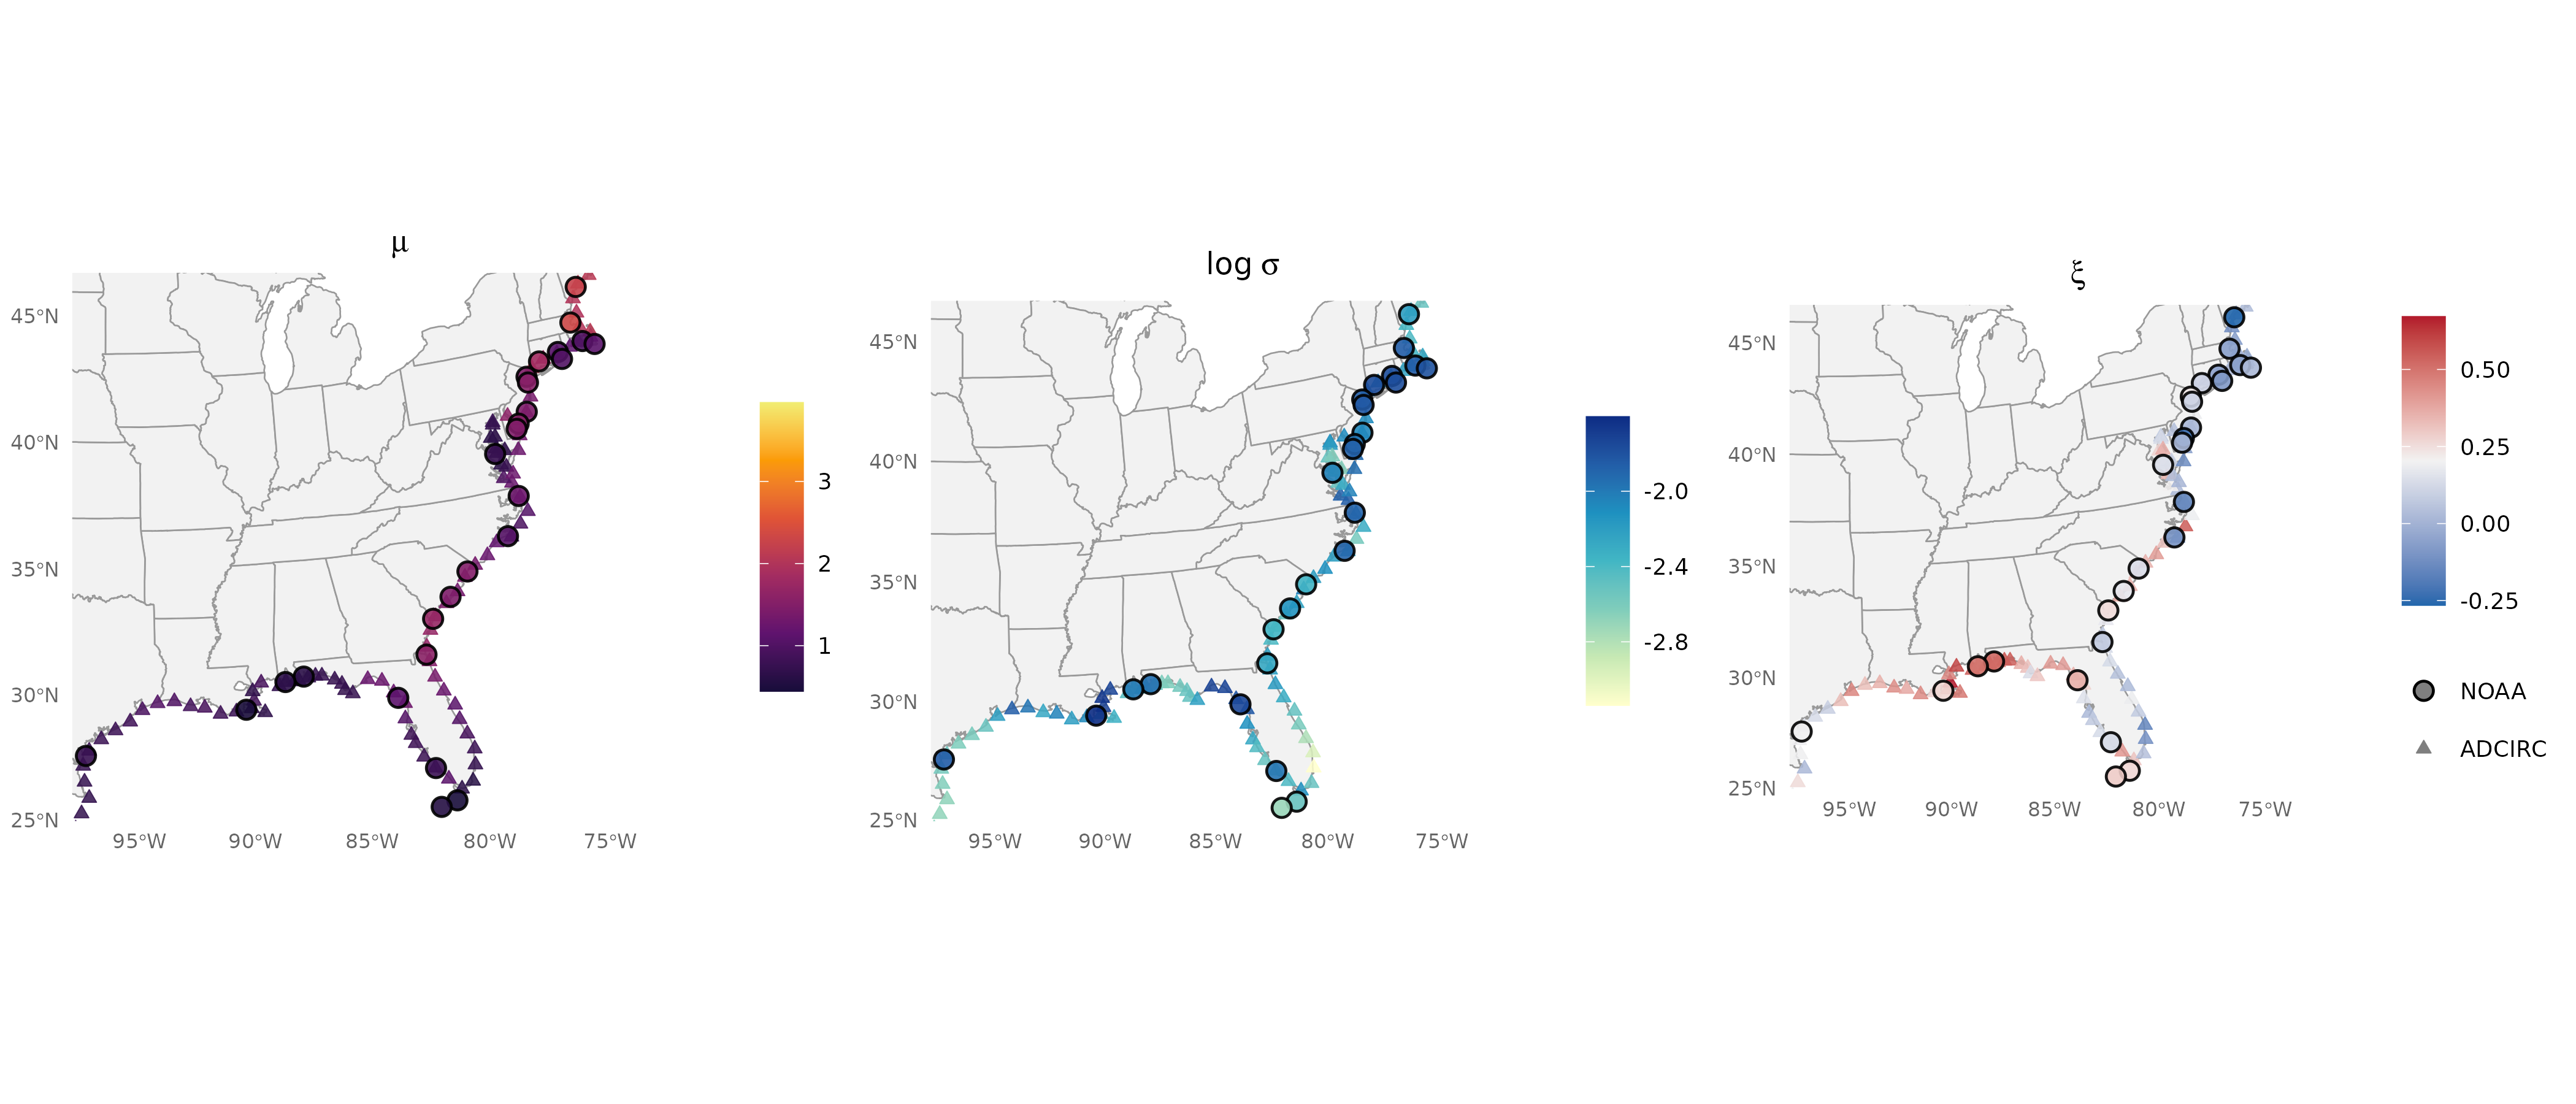
\includegraphics[width=\textwidth]{figures/stage1_mle_map.png}
\caption{Stage~1 pointwise GEV maximum likelihood estimates at 129 sites. NOAA tidal gauges (circles with black outlines) and ADCIRC simulation sites (triangles). Left: location $\hat{\mu}$ (meters). Center: log-scale $\log\hat{\sigma}$. Right: shape $\hat{\xi}$, with diverging color scale centered at zero.}
\label{fig:stage1}
\end{figure}

\subsection{Kriged NOAA GEV Parameter Fields}

Figure~\ref{fig:kriged} shows the kriged NOAA parameter predictions at the coastal grid points. The kriging produces smooth spatial fields that interpolate between and extrapolate beyond the observation sites.

\paragraph{Location $\tilde{\mu}_N$.} The kriged location field reproduces the strong south-to-north gradient observed in the raw data, ranging from 0.53\,m in the Florida Keys to 3.86\,m in Maine. The smoothness of the field reflects the long estimated range ($\rho_1 = 1659$\,km) of the dominant latent GP, confirming that mean sea level location varies gradually over large spatial scales.

\paragraph{Log-scale $\log\tilde{\sigma}_N$.} The kriged scale field ranges from $-2.38$ to $-1.83$, with higher values (greater variability) along the Gulf Coast and the mid-Atlantic. The shorter range parameters ($\rho_2 = 264$\,km) produce a field with more local variation than $\mu$, reflecting the more regionally variable nature of storm surge intensity.

\paragraph{Shape $\tilde{\xi}_N$.} The shape field ranges from $-0.10$ to 0.20 after kriging. The Gulf Coast retains elevated positive values, while the northeast Atlantic coast is near zero. Notably, the kriged shape values are substantially shrunk toward the mean ($\tilde{\beta}_3 = 0.10$) compared to the site-level estimates, which is expected given the high estimation uncertainty in $\xi$ with only $\sim$40 years of data per site.

\begin{figure}[ht]
\centering
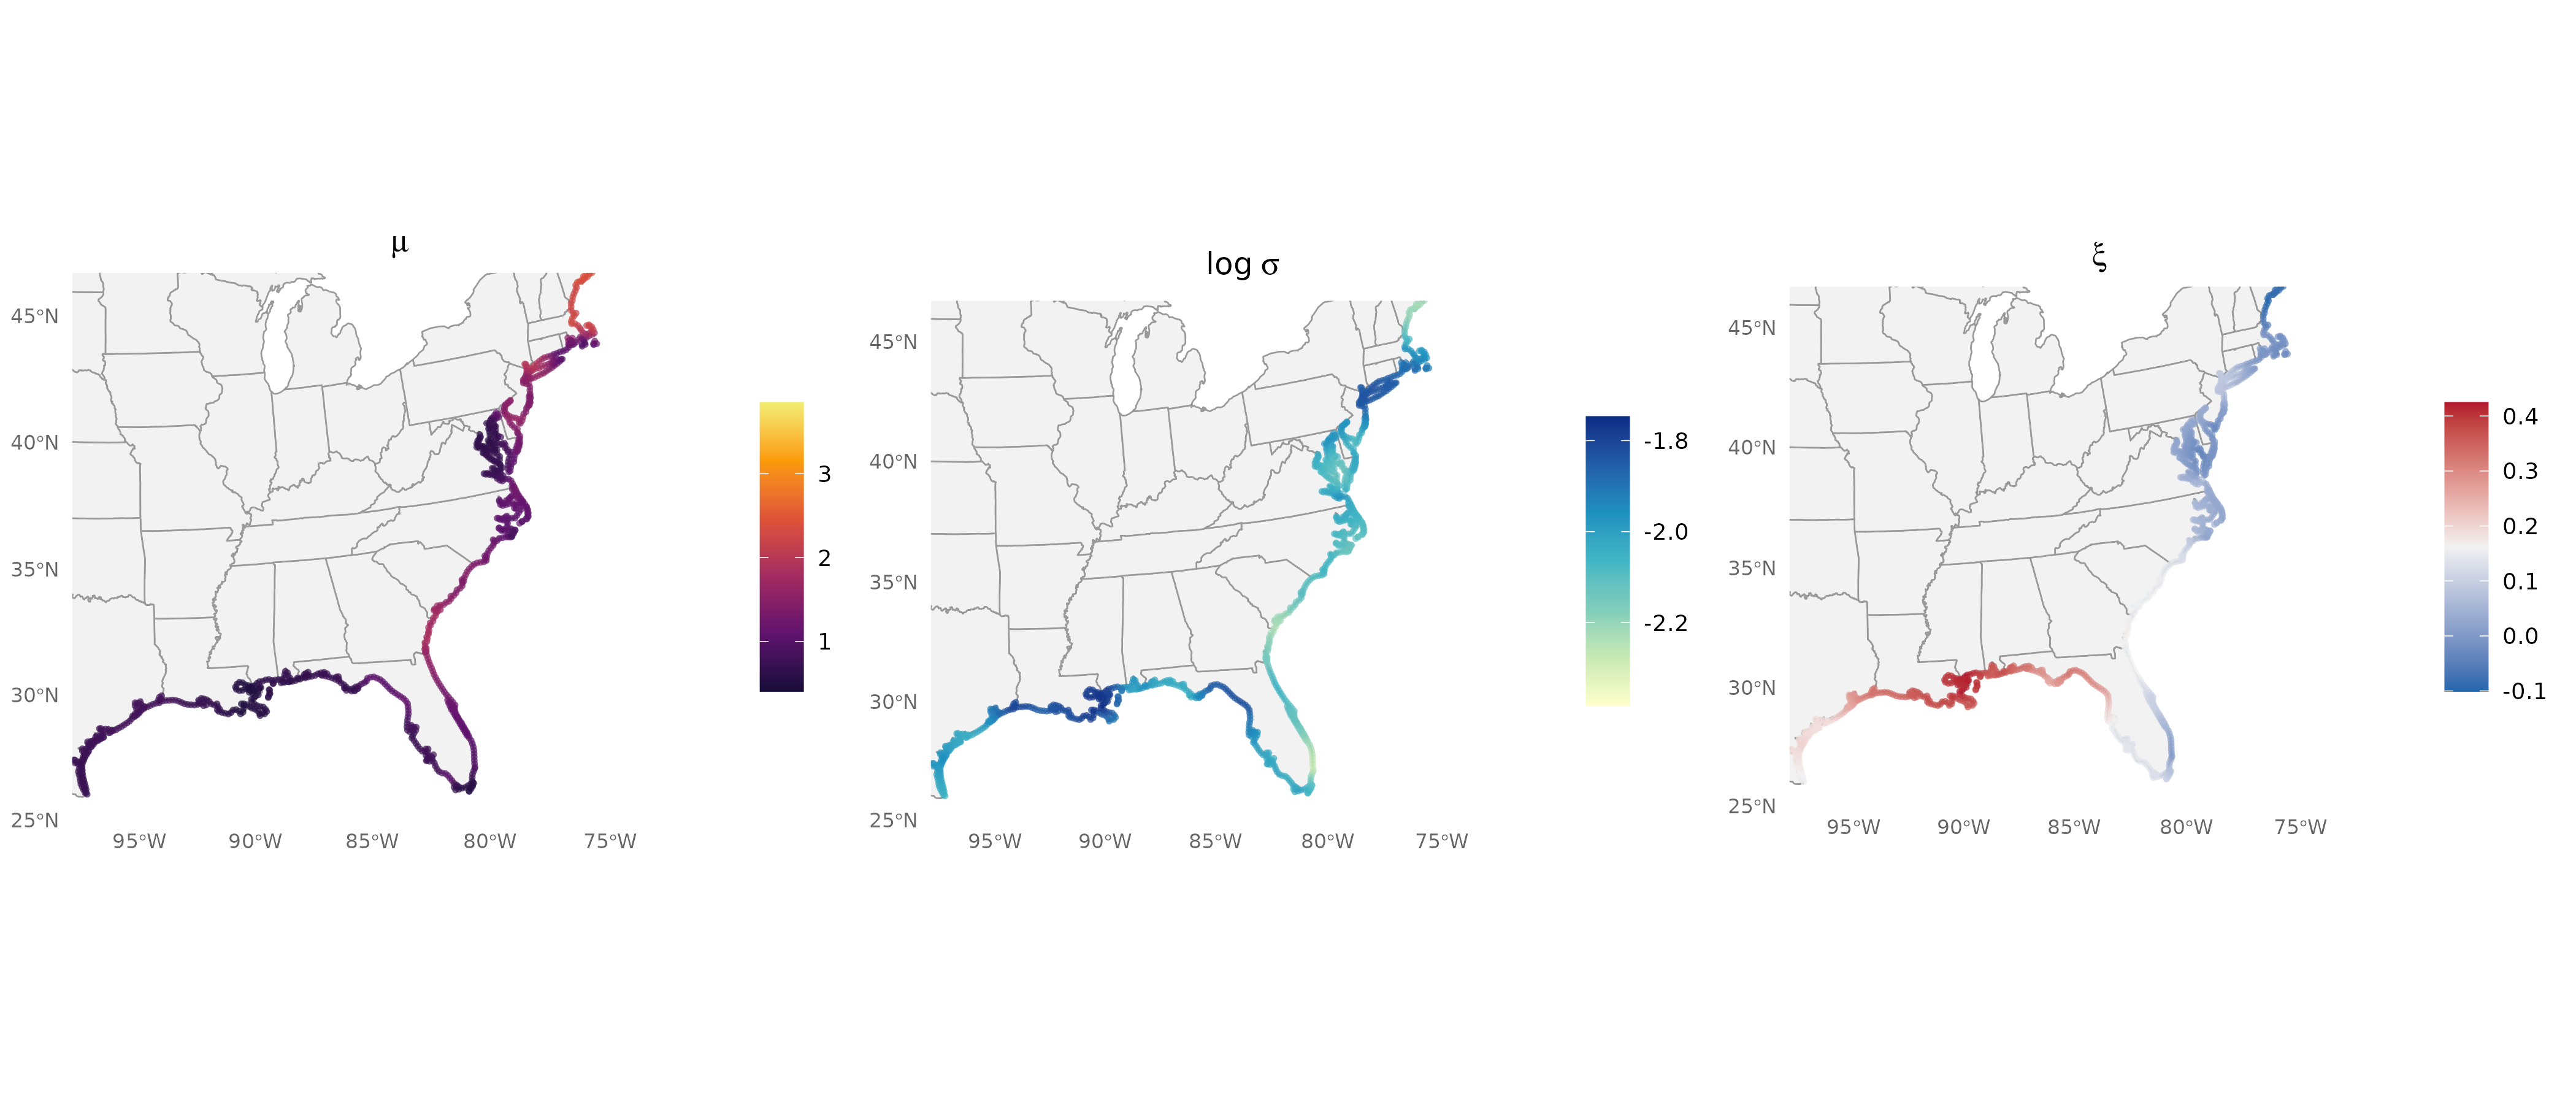
\includegraphics[width=\textwidth]{figures/kriged_params_map.png}
\caption{Kriged NOAA GEV parameter fields at coastal prediction grid points. Left: location $\tilde{\mu}_N$ (meters). Center: log-scale $\log\tilde{\sigma}_N$. Right: shape $\tilde{\xi}_N$, with diverging color scale centered at zero. The smooth spatial fields reflect the coregionalization model's estimated range parameters.}
\label{fig:kriged}
\end{figure}

\subsection{100-Year Return Levels}

Figures~\ref{fig:rl100} and~\ref{fig:rl100se} display the kriged 100-year return levels and their associated standard errors.

\paragraph{Return level map.} The 100-year return level ranges from 1.20\,m in the Gulf of Mexico and southern Florida to 4.24\,m in northern New England. The highest return levels occur along the Maine coast, driven by the combination of large tidal range (high $\mu$) and moderate tail behavior. The Gulf Coast shows intermediate return levels ($\sim$2$--$3\,m) despite lower $\mu$, reflecting the heavy-tailed GEV shape ($\xi > 0$) induced by hurricane storm surge. The NOAA site-level return level estimates (overlaid with black outlines) are broadly consistent with the kriged surface, with slight shrinkage toward the spatial mean as expected.

\paragraph{Uncertainty map.} The return level standard errors (delta method) are lowest along the Atlantic coast ($\sim$0.1$--$0.2\,m), where the observation network is densest. Uncertainty increases along the Gulf Coast ($\sim$0.3$--$0.6\,m), particularly in the Louisiana--Mississippi region. This elevated Gulf uncertainty reflects both the sparser observation network in that region and the larger $\xi$ values, which amplify return level uncertainty through the nonlinear dependence of the GEV quantile function on the shape parameter. The spatial pattern of uncertainty directly informs where additional monitoring would most reduce flood risk estimation error.

\begin{figure}[ht]
\centering
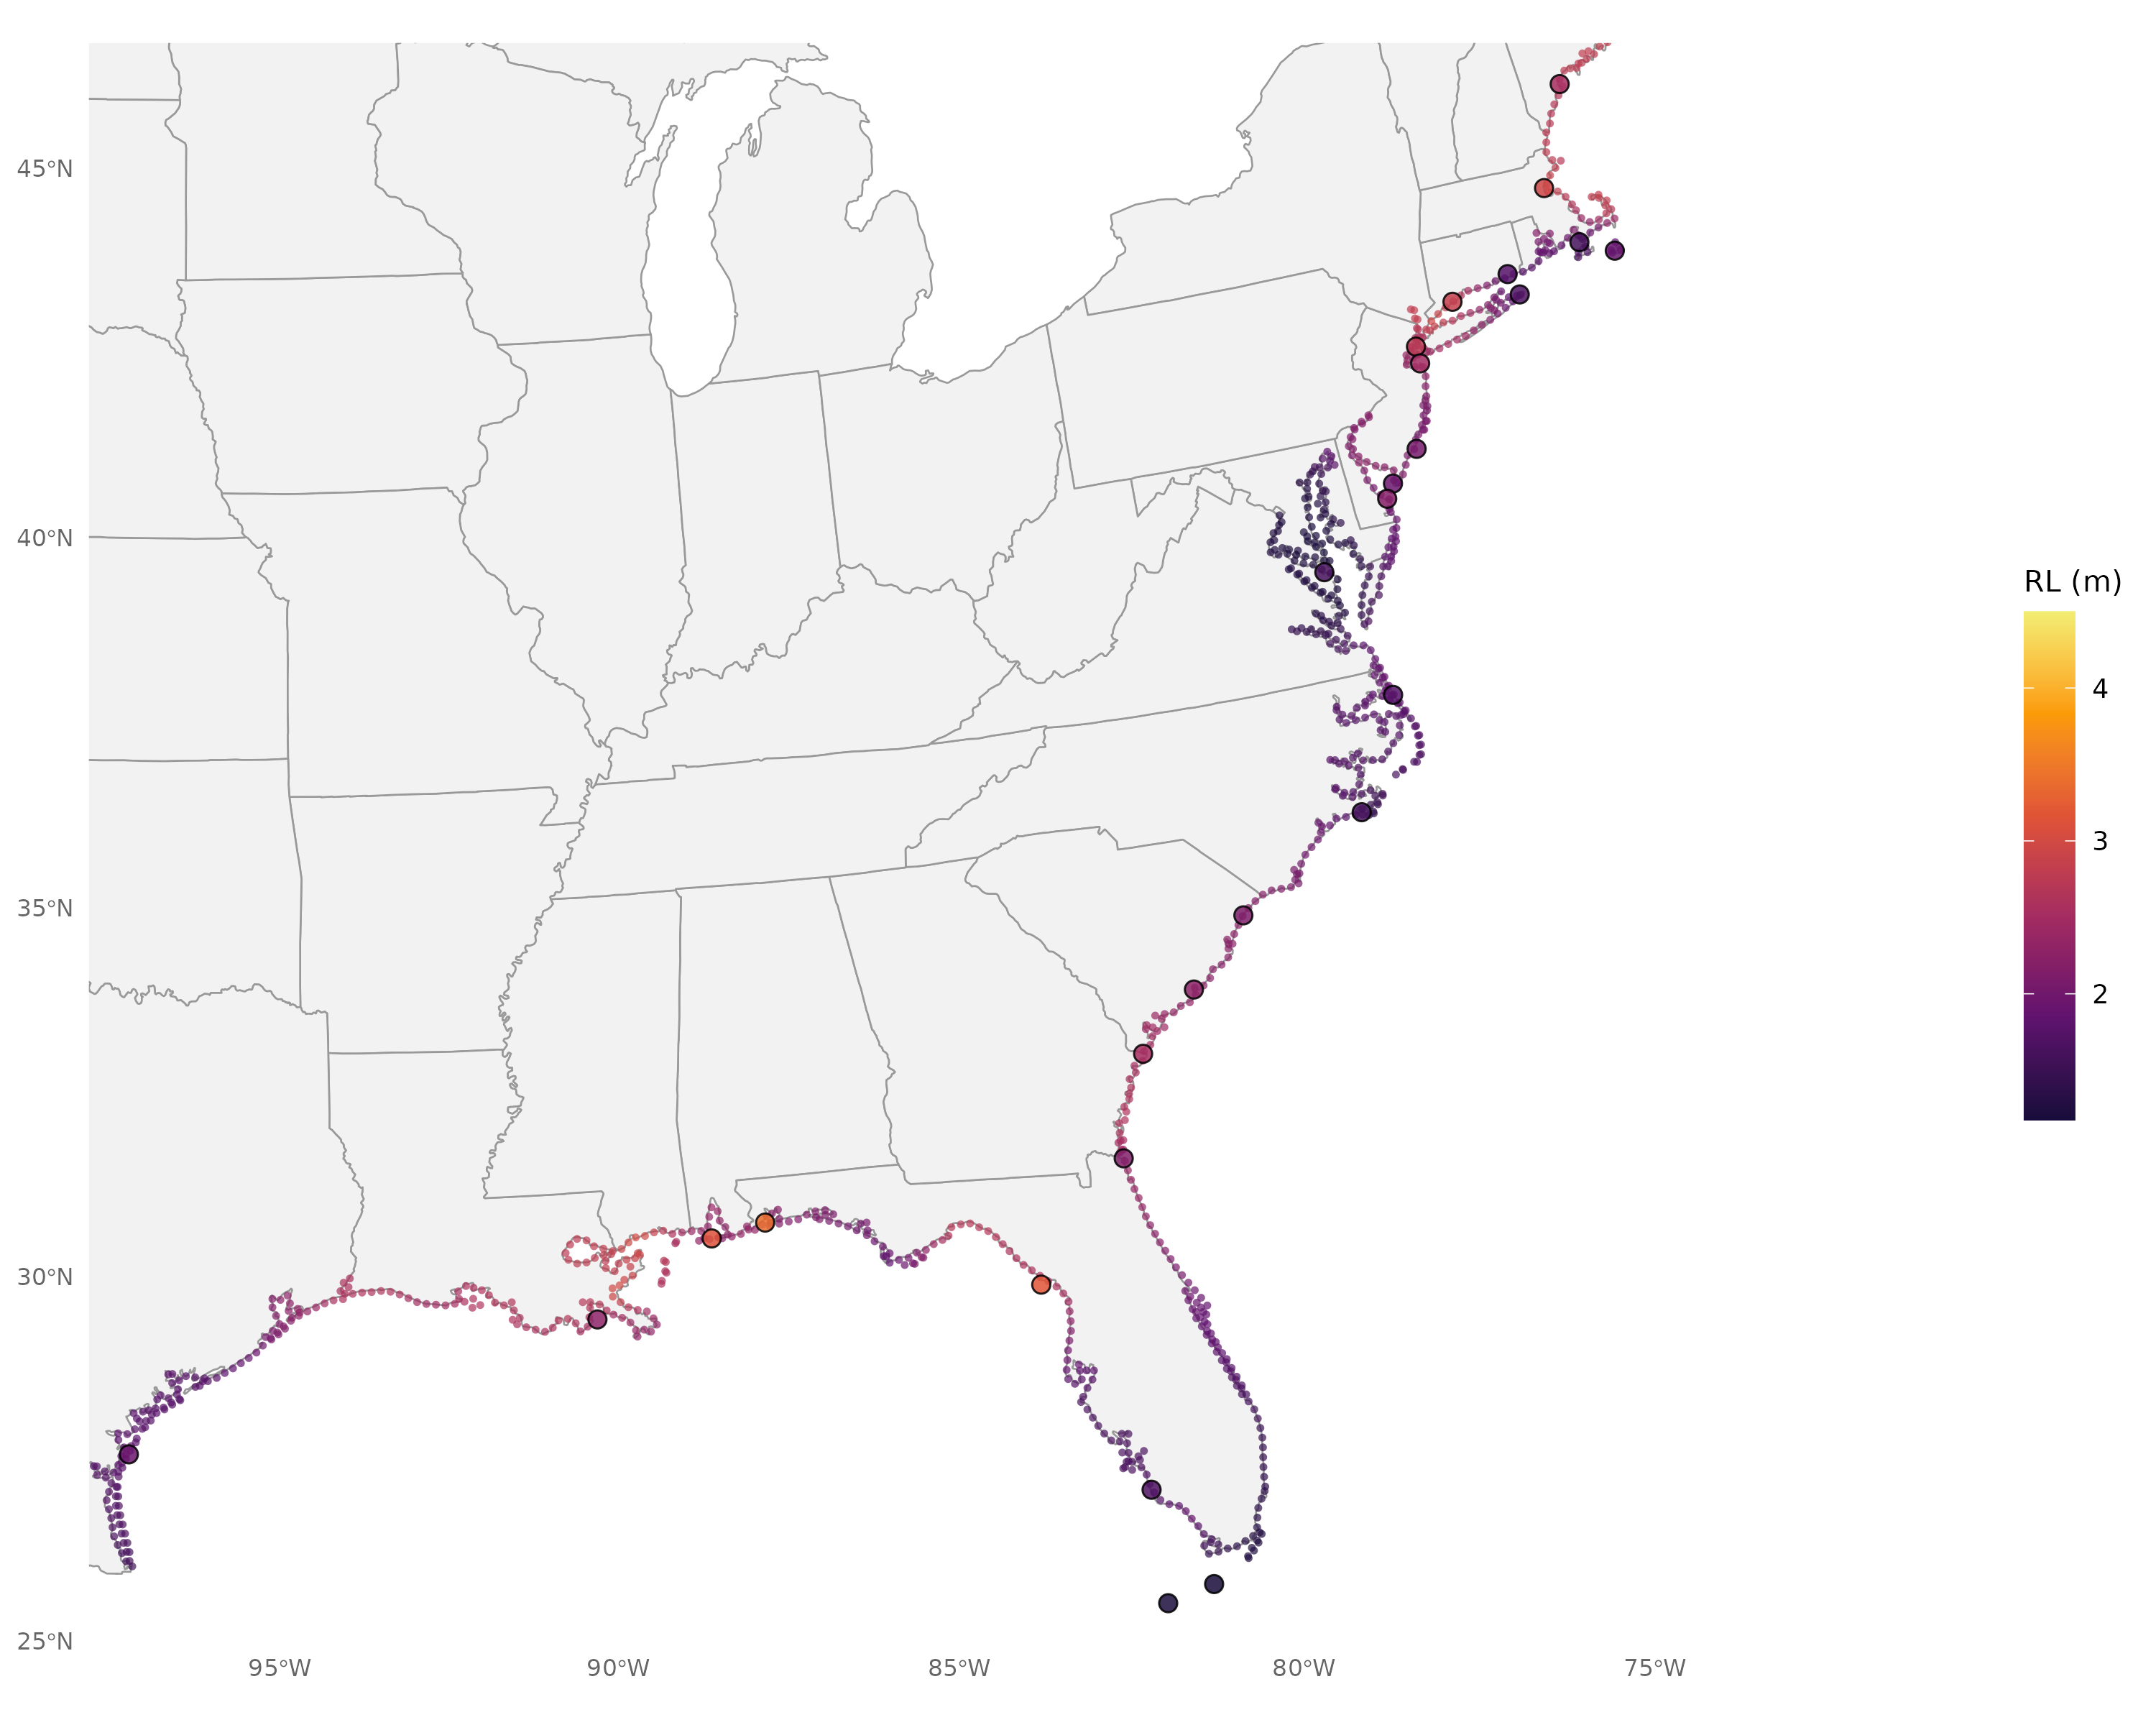
\includegraphics[width=0.75\textwidth]{figures/return_level_100yr.png}
\caption{Kriged 100-year return levels (meters) at coastal prediction grid points. NOAA site-level return level estimates are overlaid with black outlines. The highest return levels occur along the Maine coast; intermediate values along the Gulf Coast reflect heavy-tailed GEV shapes despite lower location parameters.}
\label{fig:rl100}
\end{figure}

\begin{figure}[ht]
\centering
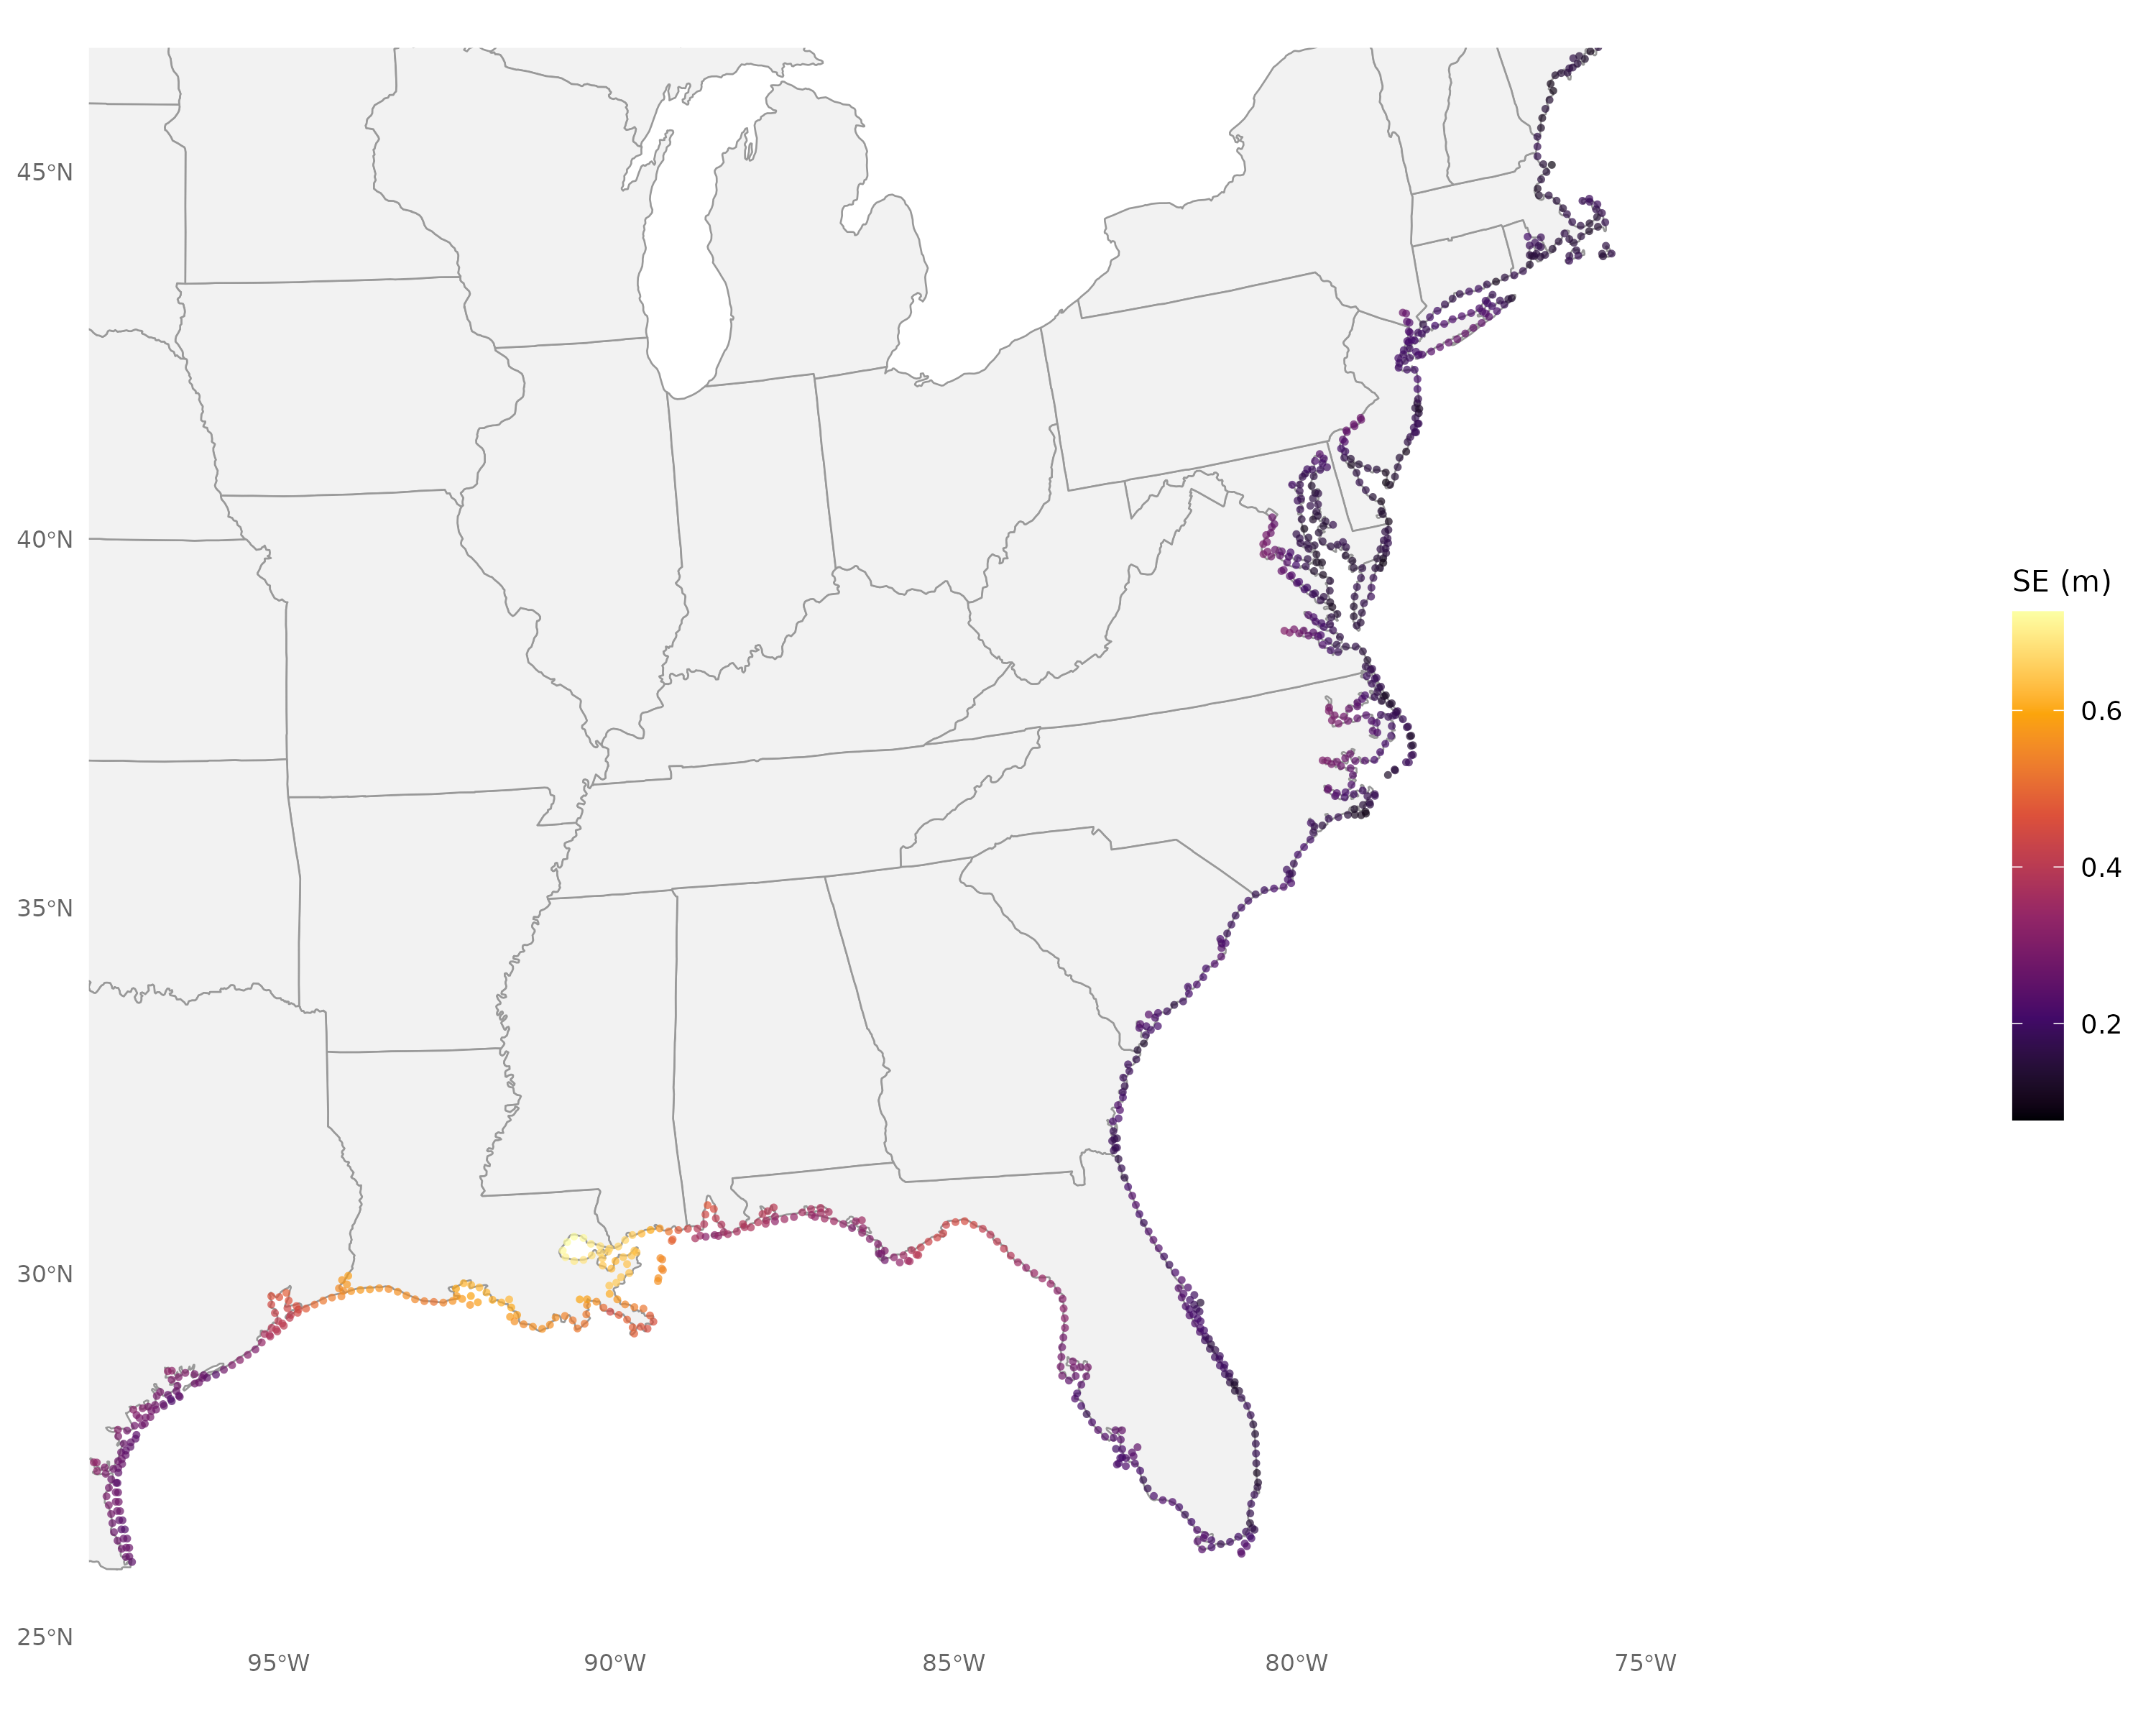
\includegraphics[width=0.75\textwidth]{figures/return_level_se.png}
\caption{Delta-method standard errors of the 100-year return level. Uncertainty is lowest along the densely observed Atlantic coast and highest in the Gulf of Mexico, where the observation network is sparser and positive $\xi$ amplifies return level uncertainty.}
\label{fig:rl100se}
\end{figure}

\begin{table}[h]
\centering
\caption{Summary of kriged NOAA GEV parameters and 100-year return levels.}
\label{tab:kriging_summary}
\begin{tabular}{@{}lcc@{}}
\toprule
& Min & Max \\
\midrule
$\tilde{\mu}_N$ (m) & 0.53 & 3.86 \\
$\log\tilde{\sigma}_N$ & $-2.38$ & $-1.83$ \\
$\tilde{\xi}_N$ & $-0.10$ & 0.20 \\
100-yr return level (m) & 1.20 & 4.24 \\
100-yr SE (m) & 0.08 & 0.75 \\
\bottomrule
\end{tabular}
\end{table}

%======================================================================
\section{Naive Model Comparisons}
\label{sec:naive}
%======================================================================

To quantify the value of data fusion, we fit two naive baseline models using the same coregionalization framework but restricted to a single data source:
\begin{itemize}[nosep]
    \item \textbf{NOAA-only}: 3-dim GP ($\mu$, $\log\sigma$, $\xi$) at 29 sites, 12 parameters.
    \item \textbf{ADCIRC-only}: 3-dim GP at 100 sites, 12 parameters.
\end{itemize}
Both models use the same bootstrap $\bW_{\text{tap}}$ (subsetted to the relevant sites) and taper range $\lambda = 300$\,km.

\subsection{Model Fit}

\begin{table}[h]
\centering
\caption{Model fit summary. The joint model's substantially lower NLL reflects the information gained by combining both data sources.}
\label{tab:model_fit}
\begin{tabular}{@{}lccrl@{}}
\toprule
Model & Sites & Parameters & NLL & $\tilde{\bm{\rho}}$ (km) \\
\midrule
Joint (6-dim) & 129 & 33 & $-103.61$ & 1659, 264, 1093, 281, 88, 2294 \\
NOAA-only & 29 & 12 & $+13.67$ & 827, 239, 1068 \\
ADCIRC-only & 100 & 12 & $-75.49$ & 2218, 380, 1213 \\
\bottomrule
\end{tabular}
\end{table}

The joint model achieves an NLL of $-103.61$, far lower than the NOAA-only model ($+13.67$), confirming the substantial information gain from incorporating ADCIRC sites. The NOAA-only model's positive NLL reflects the difficulty of fitting a spatial model with only 29 sites: the measurement error covariance $\bW$ dominates the signal covariance $\bSigma$, and the model struggles to identify spatial structure. The ADCIRC-only model ($-75.49$) performs better due to its 100 sites but cannot produce NOAA-scale return level estimates without cross-source information.

\subsection{Effect on Predictions at NOAA Sites}

Table~\ref{tab:noaa_comparison} compares kriging predictions at the 29 NOAA gauge locations against the Stage~1 MLEs. Both models produce predictions close to the site-level estimates (as expected for kriging at observed locations), but the joint model shows modest improvements in $\xi$ (RMSE 0.111 vs.\ 0.124) and 100-year return levels (RMSE 0.320 vs.\ 0.351). This reflects the ADCIRC tail information regularizing the shape parameter estimates.

\begin{table}[h]
\centering
\caption{Prediction accuracy at 29 NOAA sites: kriging predictions vs.\ Stage~1 MLEs.}
\label{tab:noaa_comparison}
\begin{tabular}{@{}lcccc@{}}
\toprule
& \multicolumn{2}{c}{RMSE} & \multicolumn{2}{c}{MAD} \\
\cmidrule(lr){2-3} \cmidrule(lr){4-5}
Parameter & Joint & NOAA-only & Joint & NOAA-only \\
\midrule
$\mu$ & 0.032 & 0.030 & 0.019 & 0.019 \\
$\log\sigma$ & 0.175 & 0.169 & 0.120 & 0.126 \\
$\xi$ & 0.111 & 0.124 & 0.093 & 0.106 \\
100-yr RL & 0.320 & 0.351 & 0.194 & 0.208 \\
\bottomrule
\end{tabular}
\end{table}

\subsection{Uncertainty Reduction}

The primary benefit of fusion is uncertainty reduction. Table~\ref{tab:se_comparison} shows that the joint model reduces mean return level SE by 35\% overall relative to NOAA-only (0.261 vs.\ 0.403\,m). The improvement is largest along the Atlantic coast (44\% reduction) and substantial in the Gulf (25\% reduction).

\begin{table}[h]
\centering
\caption{Mean standard error of 100-year return levels by region.}
\label{tab:se_comparison}
\begin{tabular}{@{}lccc@{}}
\toprule
Region & Joint & NOAA-only & ADCIRC-only \\
\midrule
Overall & 0.261 & 0.403 & 0.241 \\
Atlantic ($\text{lon} > -82^\circ$) & 0.184 & 0.330 & 0.202 \\
Gulf ($\text{lon} \leq -82^\circ$) & 0.402 & 0.536 & 0.312 \\
\bottomrule
\end{tabular}
\end{table}

The SE ratio (NOAA-only / joint) has a median of 1.59 and mean of 1.71, with 57\% of grid points showing ratios above 1.5 and 25\% above 2.0 (uncertainty halved or better). The largest gains (ratio up to 4.8) occur along Florida's Atlantic coast, where dense ADCIRC coverage fills the gap between sparse NOAA gauges (Figure~\ref{fig:se_ratio}).

\subsection{Effect on Point Estimates}

While the primary benefit of fusion is uncertainty reduction, the return level point estimates also change in physically meaningful ways. Figure~\ref{fig:rl_ratio} shows the ratio of joint to NOAA-only return levels. Most of the coast shows ratios near 1.0 (changes within $\pm$10\%), confirming that fusion does not drastically alter the return level surface. The Gulf Coast shows modest increases (ratio $\sim$1.1--1.3), driven by ADCIRC's positive $\xi$ information raising return levels in that region. The Chesapeake Bay area shows slight decreases (ratio $\sim$0.85--0.95). This pattern is consistent with the scatter plot (Figure~\ref{fig:scatter}): fusion primarily affects the shape parameter, which has a larger impact on return levels in regions where $\xi > 0$.

\begin{figure}[ht]
\centering
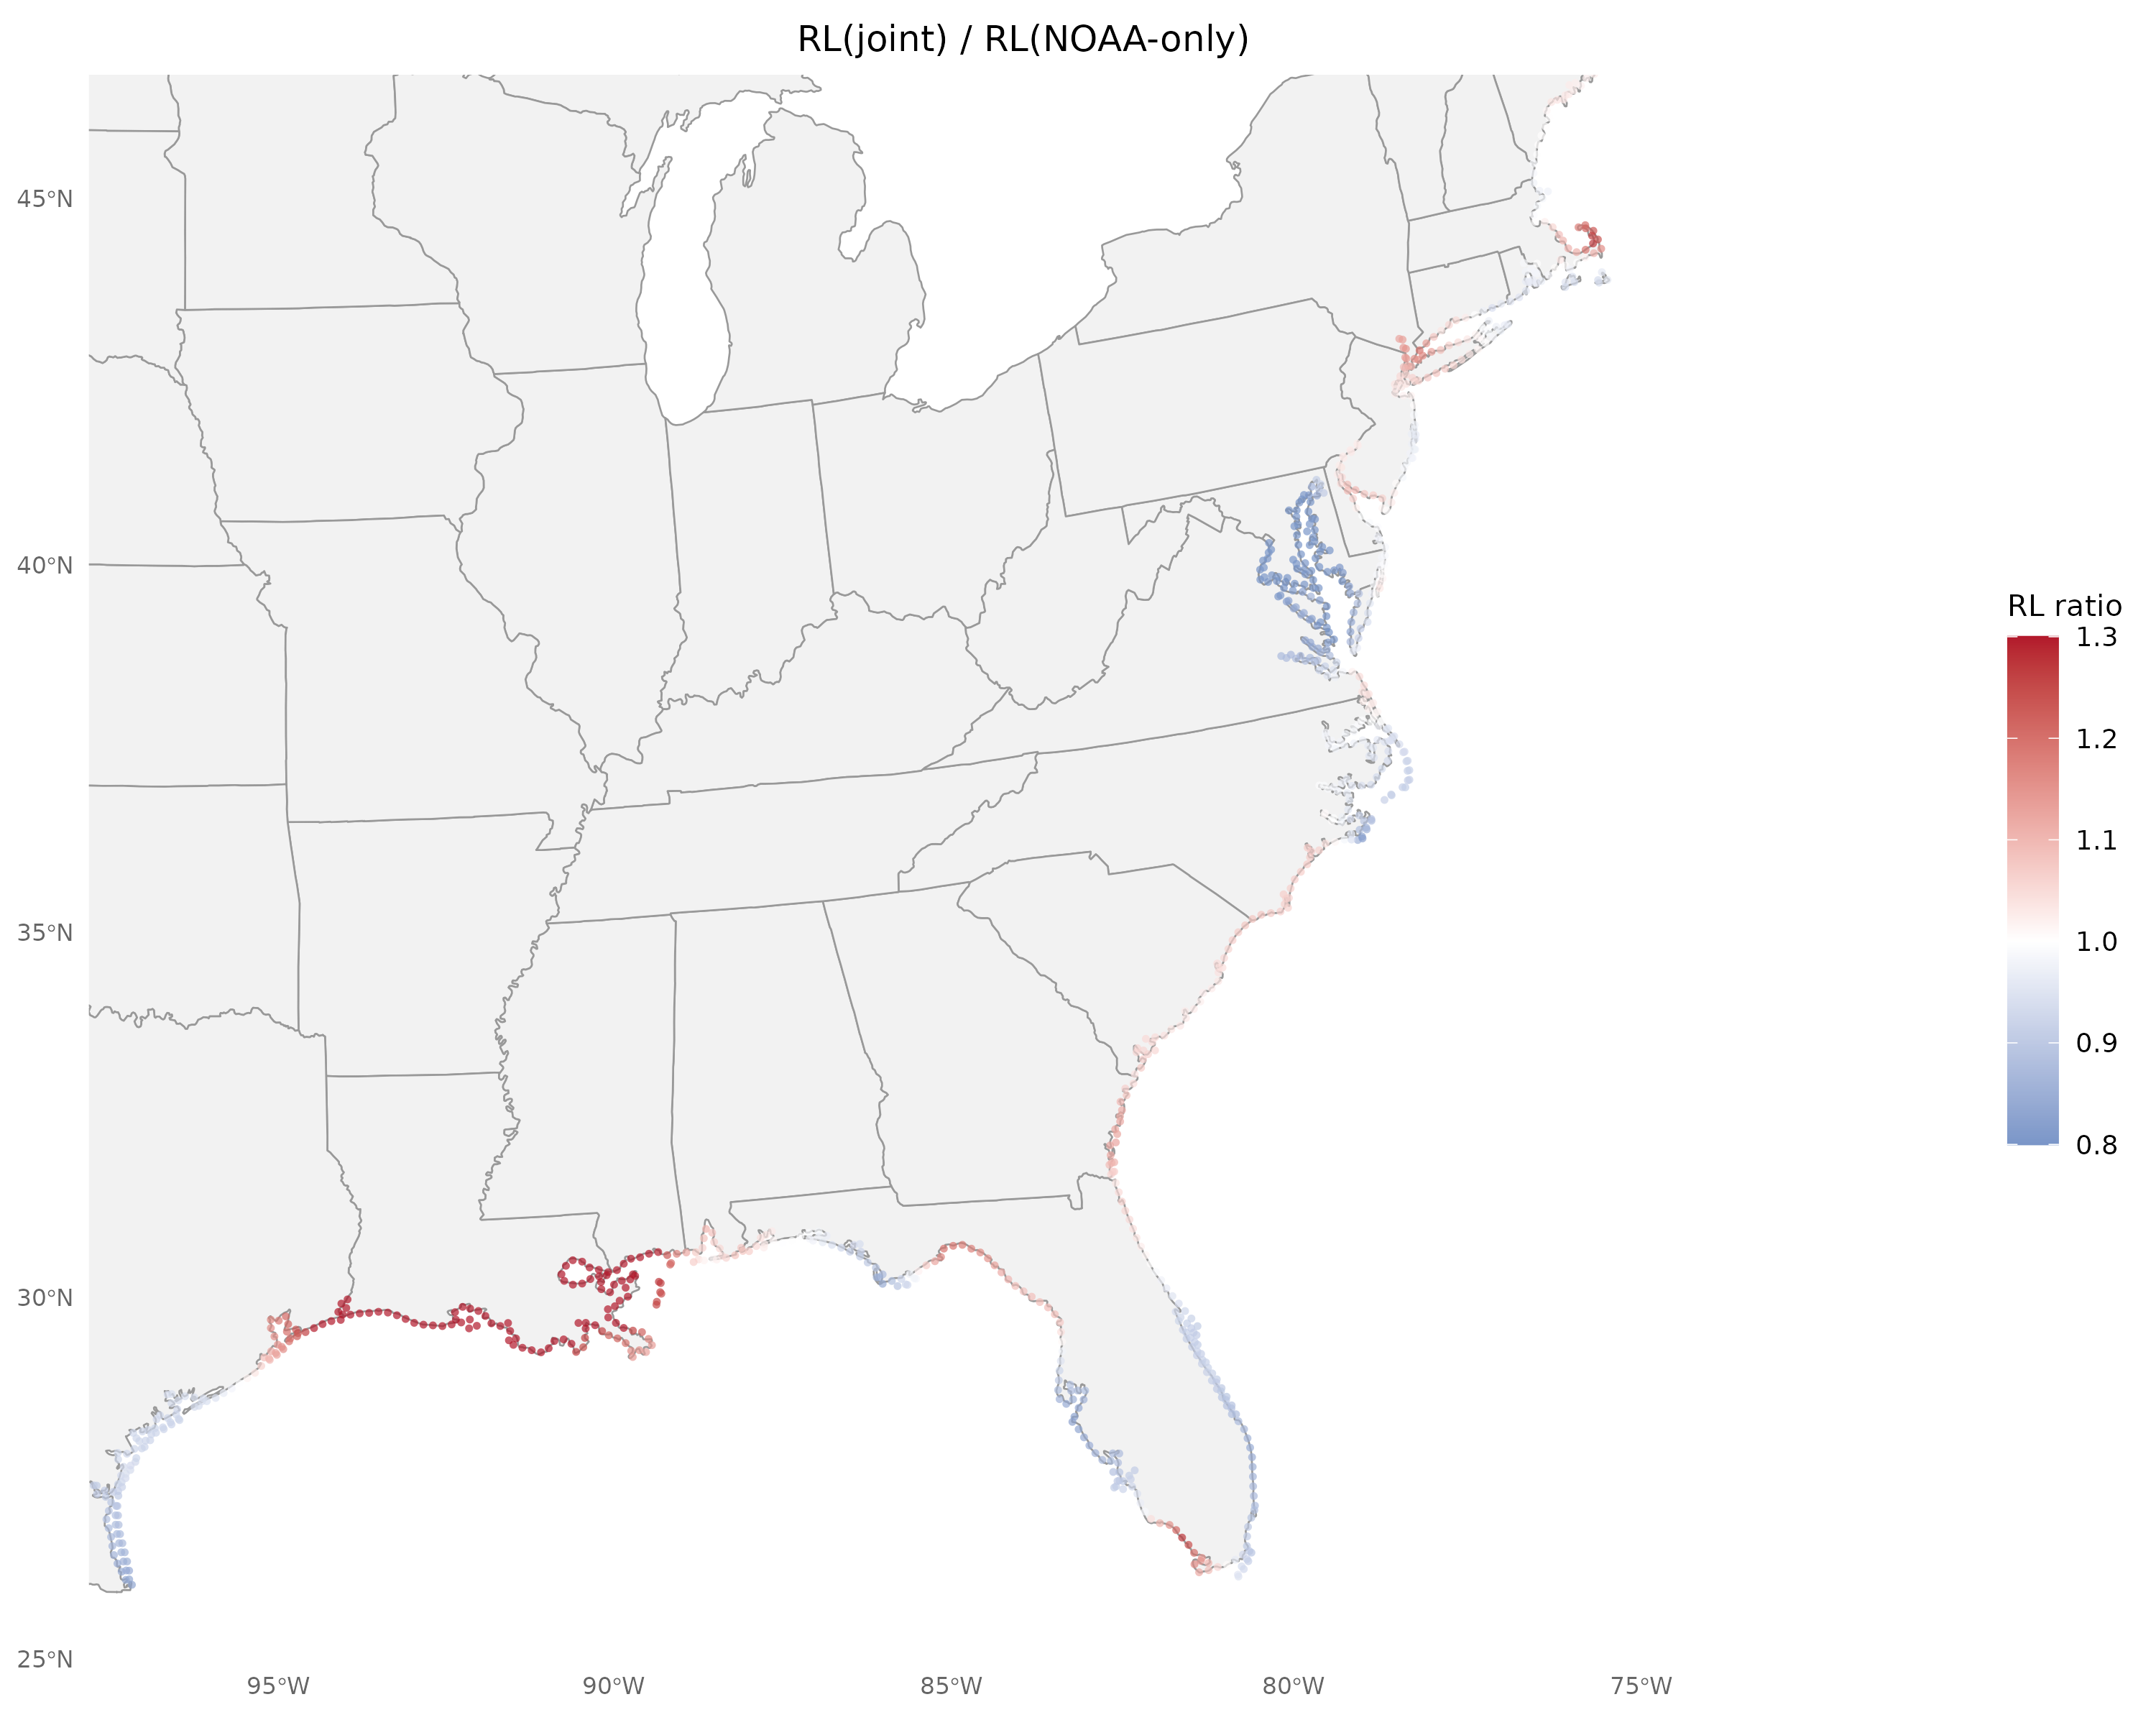
\includegraphics[width=0.75\textwidth]{figures/rl_ratio_map.png}
\caption{Ratio of 100-year return levels: RL(joint) / RL(NOAA-only). Values near 1 (white) indicate agreement; red indicates the fusion model predicts higher return levels. The Gulf Coast shows modest increases driven by ADCIRC's heavier-tailed shape parameter estimates.}
\label{fig:rl_ratio}
\end{figure}

\begin{figure}[ht]
\centering
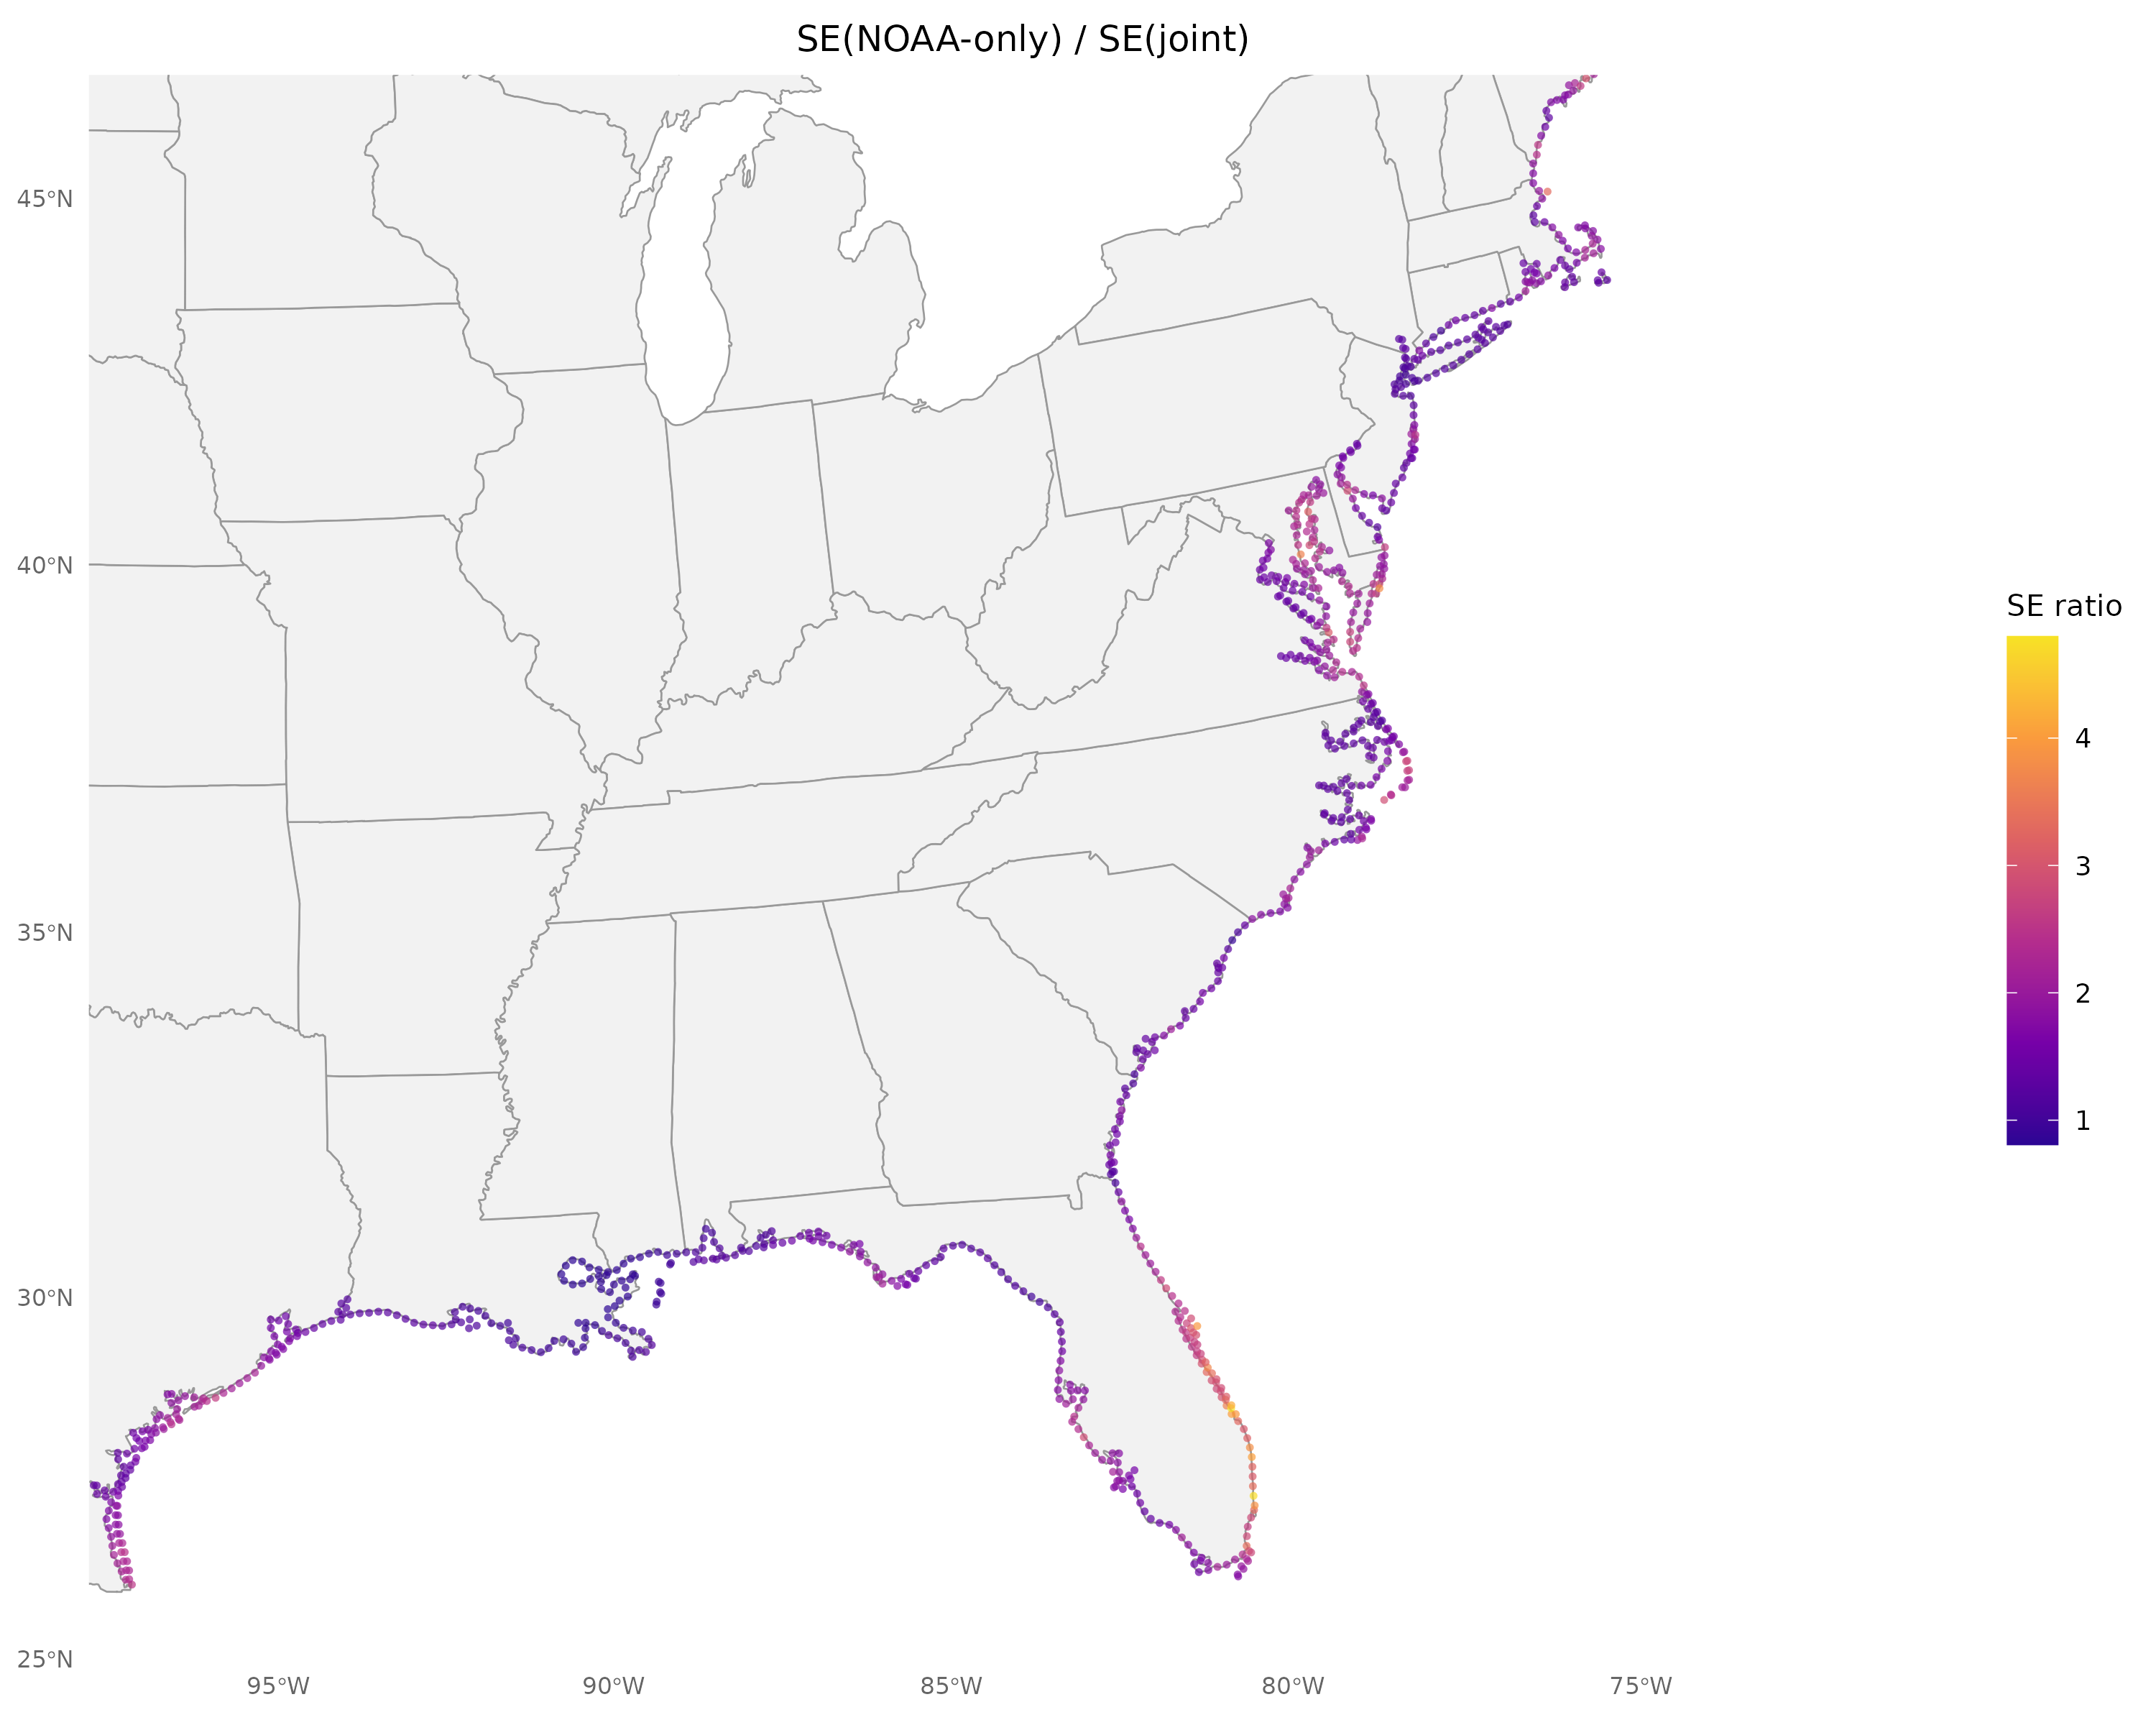
\includegraphics[width=0.75\textwidth]{figures/se_ratio_map.png}
\caption{Ratio of return level standard errors: SE(NOAA-only) / SE(joint). Values above 1 indicate the fusion model has lower uncertainty. The largest improvements occur along Florida's Atlantic coast, where ADCIRC sites fill gaps between sparse NOAA gauges.}
\label{fig:se_ratio}
\end{figure}

\begin{figure}[ht]
\centering
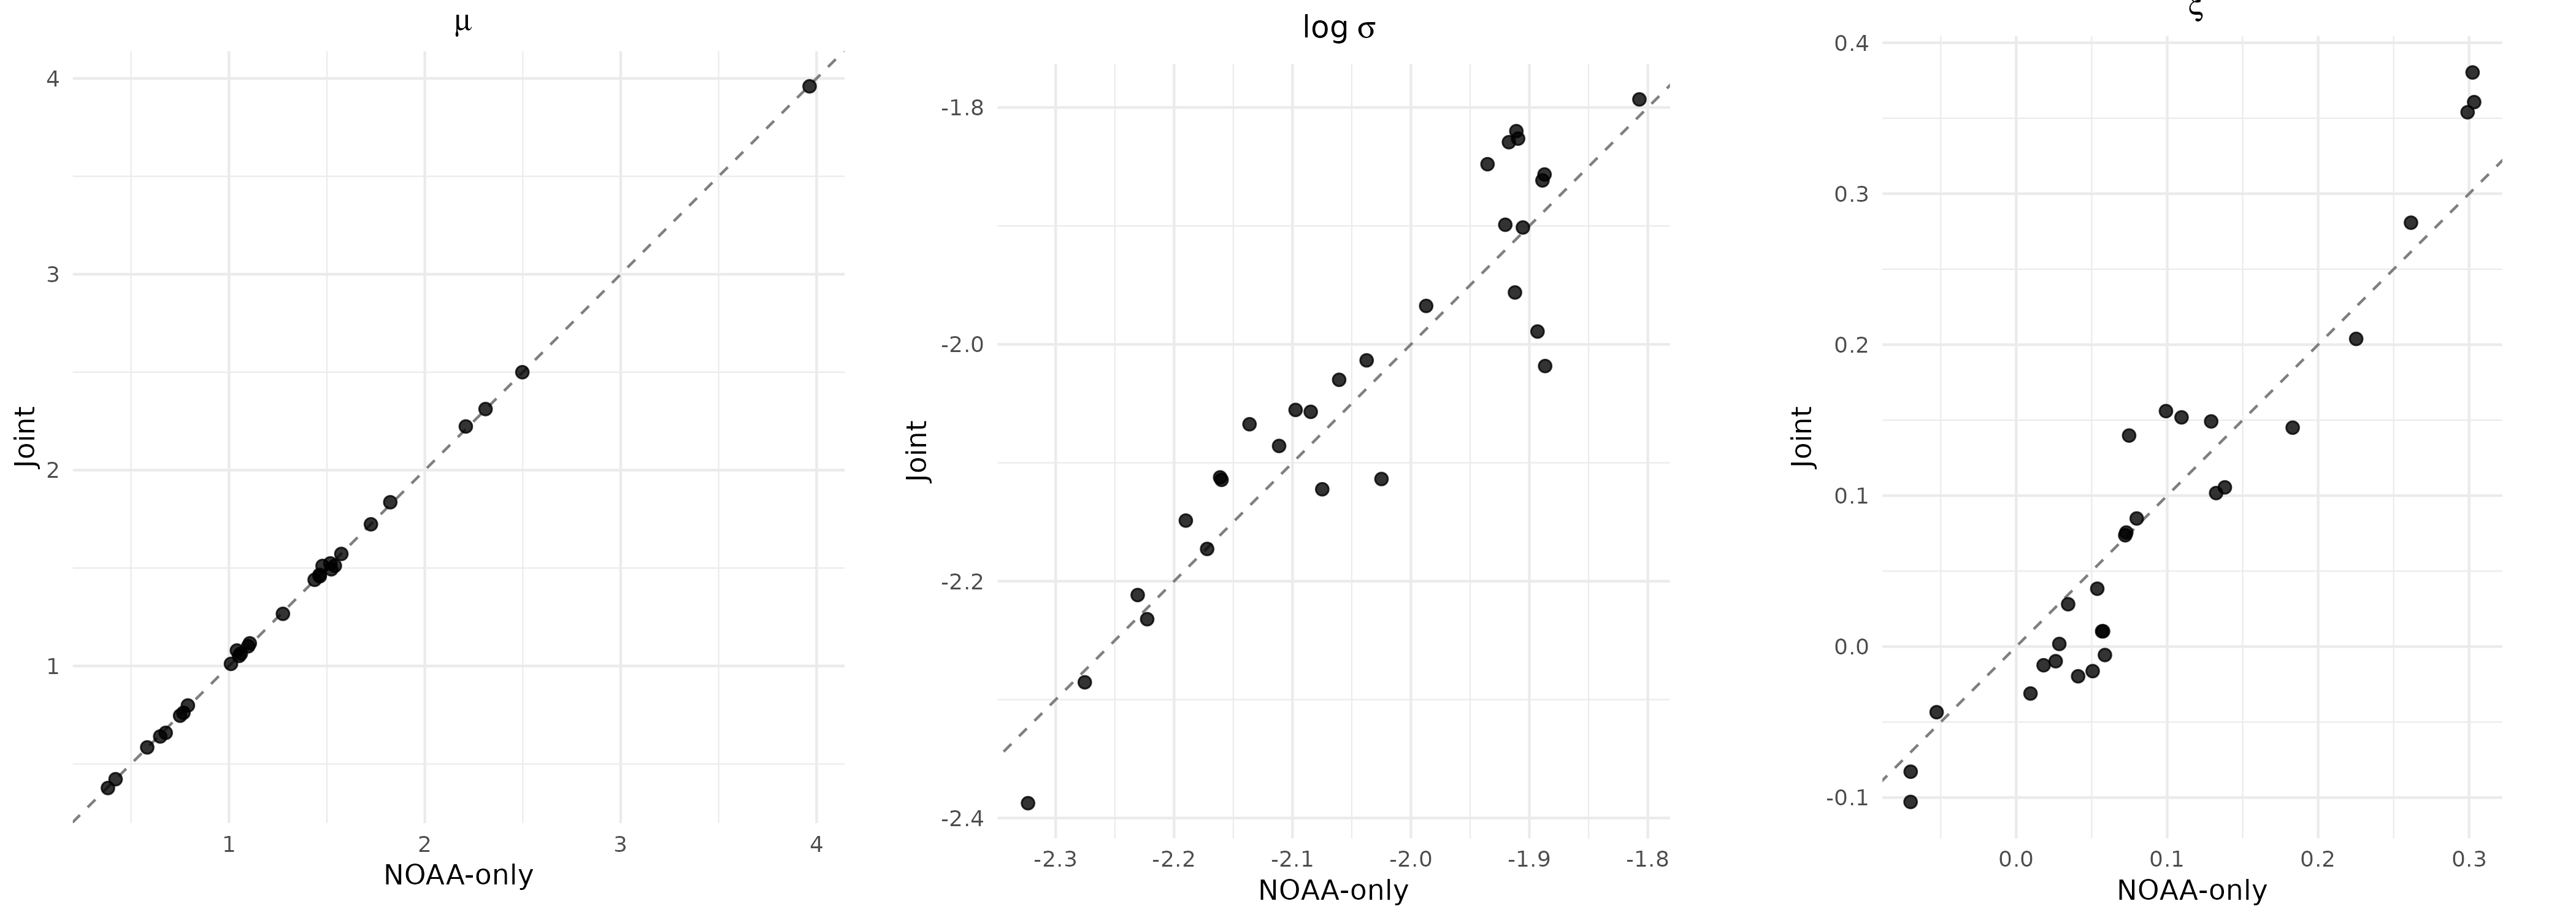
\includegraphics[width=\textwidth]{figures/noaa_site_comparison.png}
\caption{Joint vs.\ NOAA-only kriging predictions at the 29 NOAA gauge sites. The $\mu$ panel shows near-perfect agreement. The $\log\sigma$ panel shows a systematic upward shift: ADCIRC data pulls scale estimates higher. The $\xi$ panel shows the largest deviations: the joint model pulls several near-zero or negative $\hat{\xi}$ estimates toward positive values, reflecting ADCIRC's heavy-tail information flowing into the NOAA predictions.}
\label{fig:scatter}
\end{figure}

\begin{figure}[ht]
\centering
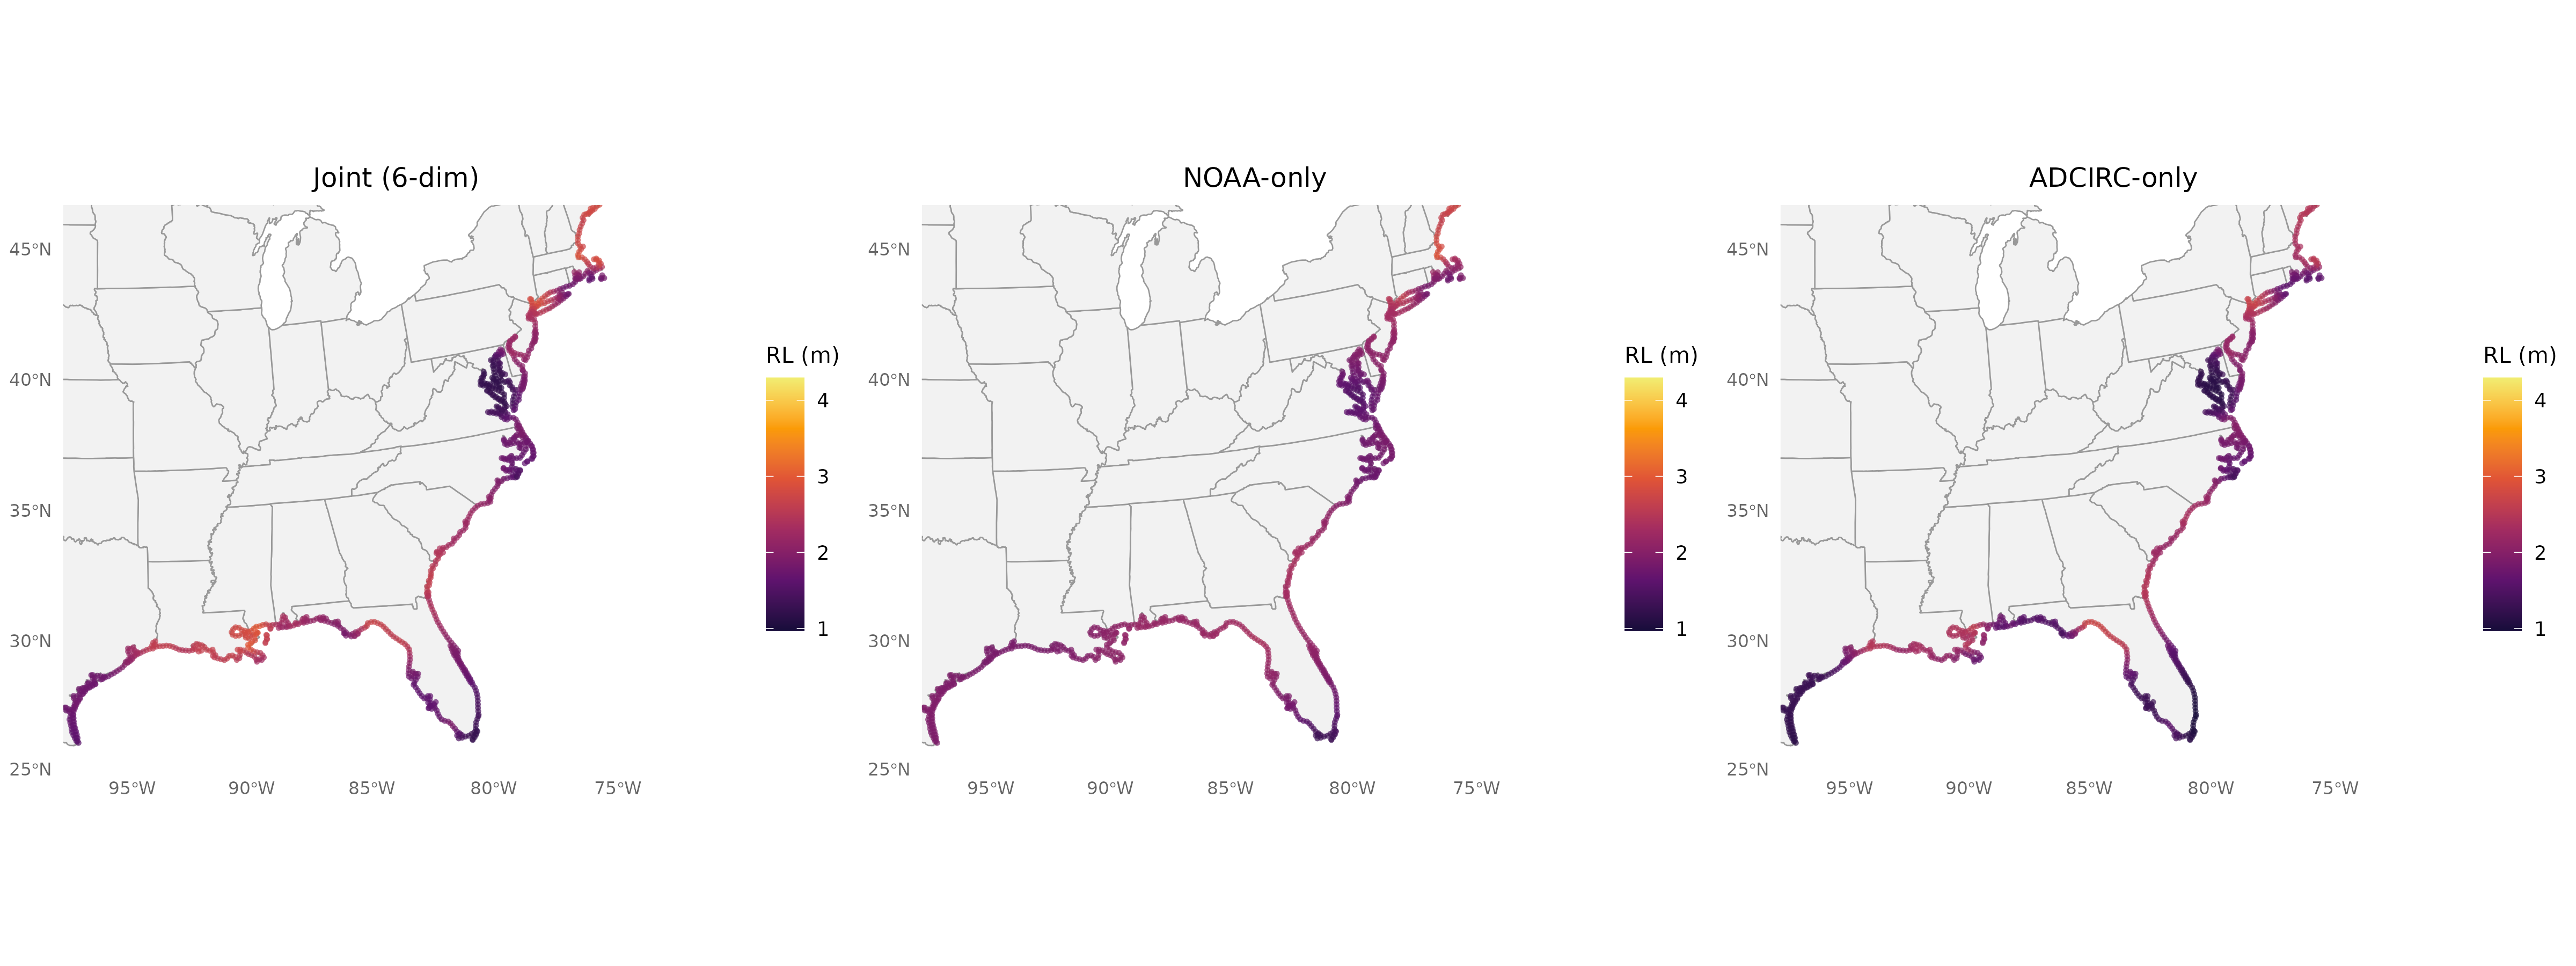
\includegraphics[width=\textwidth]{figures/comparison_return_levels.png}
\caption{100-year return levels from the three models on a common color scale. The joint and NOAA-only models produce similar spatial patterns along the Atlantic coast; the ADCIRC-only model shows systematically lower return levels in the northeast.}
\label{fig:comparison_rl}
\end{figure}

\begin{figure}[ht]
\centering
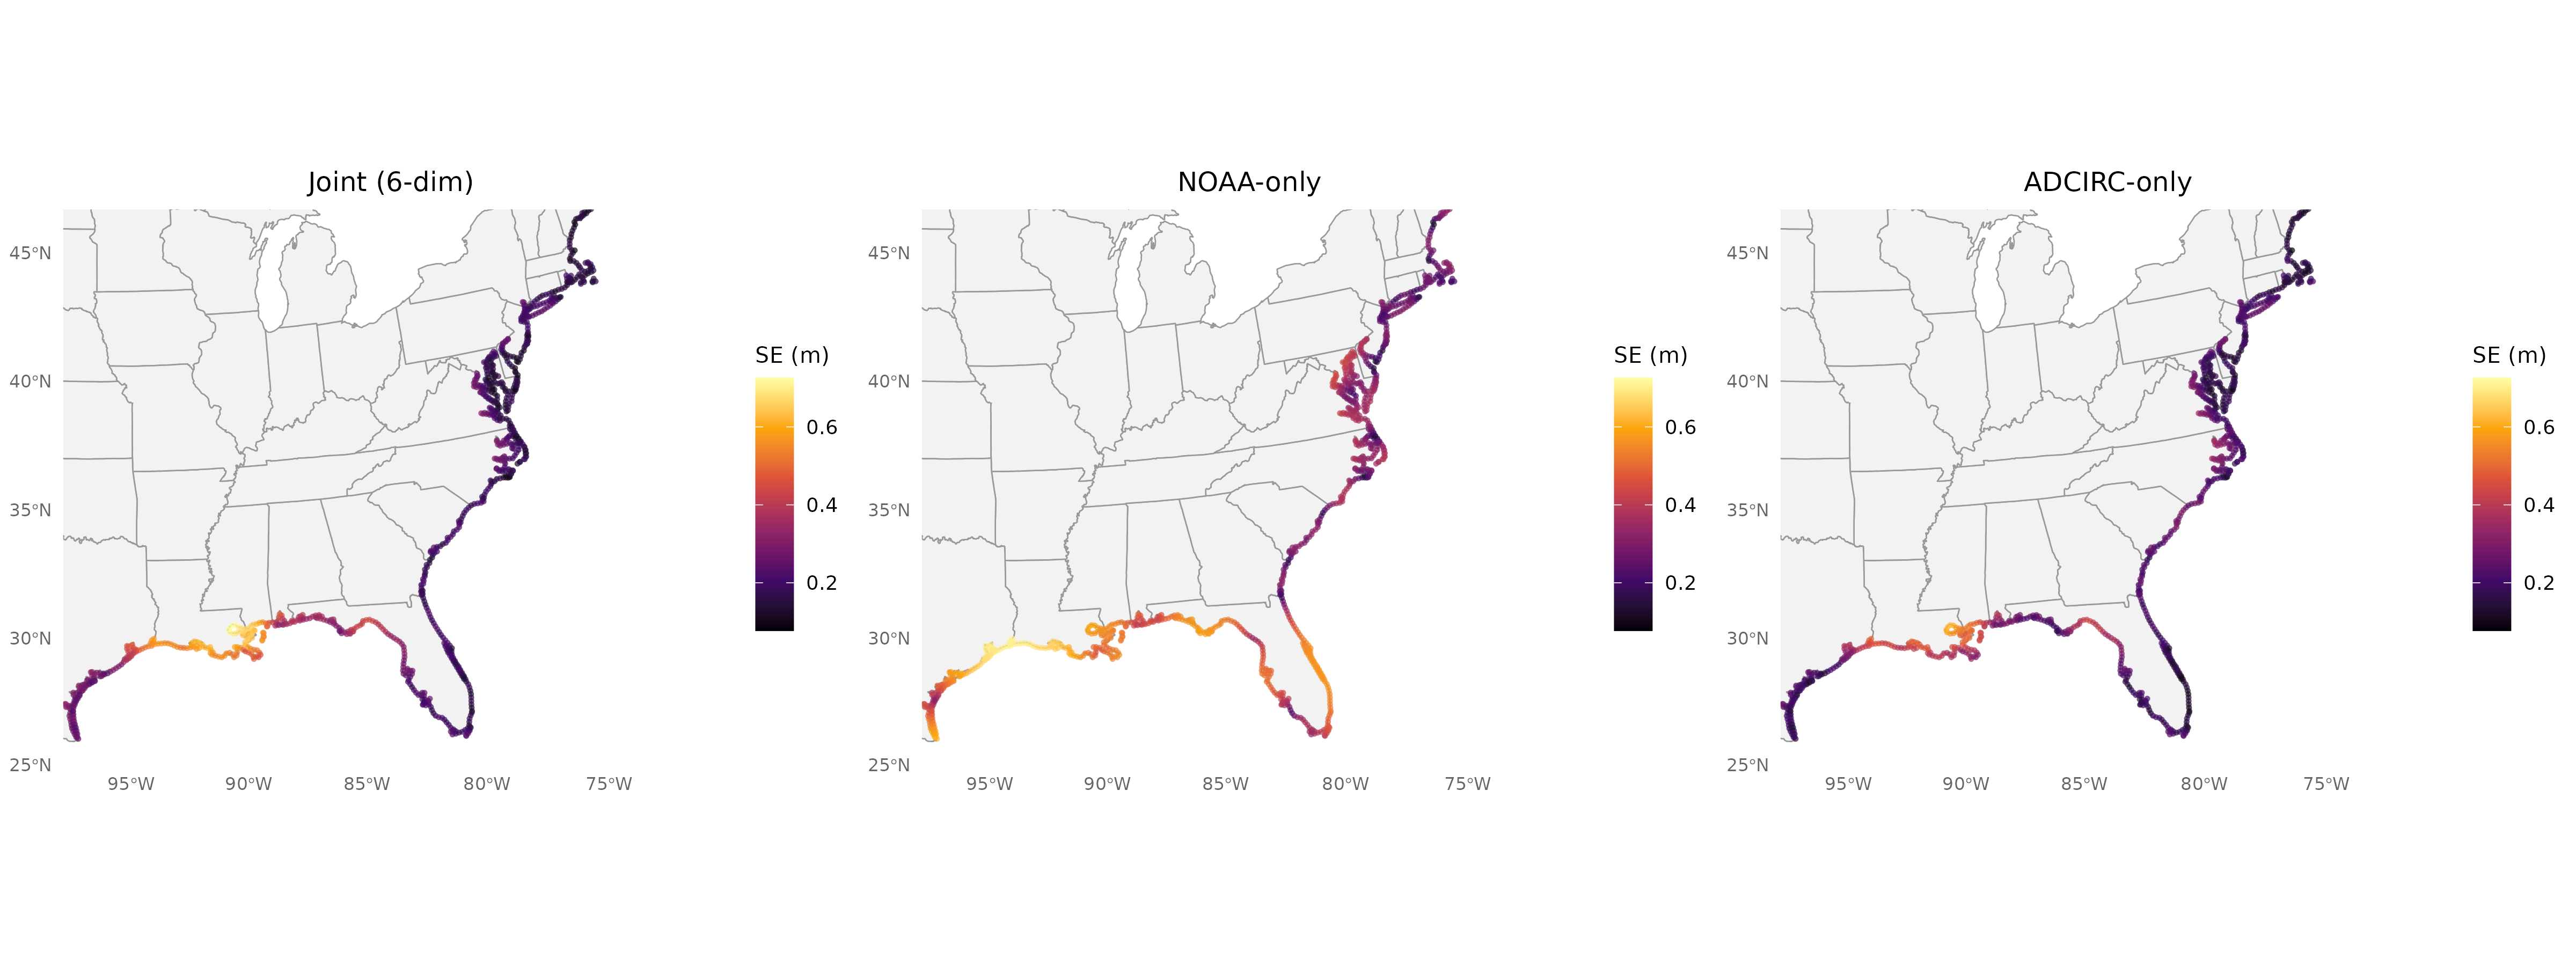
\includegraphics[width=\textwidth]{figures/comparison_se.png}
\caption{Return level standard errors from the three models on a common color scale. The NOAA-only model shows substantially higher uncertainty throughout, particularly in the Gulf and along the Southeast Atlantic coast.}
\label{fig:comparison_se}
\end{figure}

%======================================================================
\section{Implementation Summary}
%======================================================================

\begin{table}[h]
\centering
\begin{tabular}{@{}lll@{}}
\toprule
\textbf{Module} & \textbf{File} & \textbf{Status} \\
\midrule
Data loading \& distances & \texttt{R/data.R} & \checkmark\ Working \\
Stage 1 GEV fitting & \texttt{R/gev.R} & \checkmark\ All 129 sites converge \\
Covariance functions & \texttt{R/covariance.R} & \checkmark\ Tests pass \\
Bootstrap for $\bW$ & \texttt{R/bootstrap.R} & \checkmark\ $B=500$ validated \\
Stage 2 MLE (analytic gradient) & \texttt{R/spatial\_model.R} & \checkmark\ Converged, 10s \\
$\bW$ embedding & \texttt{R/spatial\_model.R} & \checkmark\ Auto-detected \\
Multi-start optimization & \texttt{scripts/multi\_start.R} & \checkmark\ 20 starts completed \\
Naive baselines & \texttt{R/naive\_model.R} & \checkmark\ NOAA-only \& ADCIRC-only \\
Prediction grid & \texttt{data-raw/prediction\_grid.csv} & \checkmark\ Filtered coastal grid \\
Kriging & \texttt{R/kriging.R} & \checkmark\ Full coast predicted \\
Return levels & \texttt{R/return\_levels.R} & \checkmark\ 100-yr computed \\
Visualization & \texttt{scripts/plot\_results.R} & \checkmark\ 5 diagnostic figures \\
Unit tests & \texttt{tests/testthat/} & 33 tests passing \\
\bottomrule
\end{tabular}
\end{table}

%======================================================================
\section{Planned Work}
%======================================================================

\begin{enumerate}[nosep]
    \item \textbf{Naive model comparisons}: Fit NOAA-only (3-dim GP, 29 sites) and ADCIRC-only (3-dim GP, 100 sites) models for comparison.
    \item \textbf{Validation}: Closed-form kriging LOO-CV at the 29 NOAA sites under all three models (joint, NOAA-only, ADCIRC-only). Metrics: LOO-RMSE and LOO-CRPS on GEV parameters and derived return levels. Reference: Rasmussen \& Williams (2006) \S5.4.2; Cressie (1993).
    \item \textbf{Trend diagnostics}: Test for temporal trends in annual maxima at each site (Mann-Kendall test, GEV with linear time trend in $\mu$).
    \item \textbf{Taper sensitivity}: Report results for $\lambda \in \{75, 150, 300\}$ using the same $\bW_{\text{bs}}$.
    \item \textbf{Covariate extension}: Incorporate SST or time trend in GEV parameters for forecasting under climate scenarios.
    \item \textbf{Visualization}: Comparison maps (fusion vs.\ naive ratio maps, LOO error maps).
    \item \textbf{Manuscript}: Target Environmetrics.
\end{enumerate}

\end{document}
